\section{Hashed Shading Algorithm}

\begin{figure}[t]
  \usetikzlibrary{shapes.arrows, fadings}
  \definecolor{LightColor}{rgb}{1.0,0.901,0.805}

  \definecolor{tile0}{HTML}{DABDE4}
  \definecolor{tile1}{HTML}{B8DBF4}
  \definecolor{tile2}{HTML}{B5EDCD}
  \definecolor{tile3}{HTML}{FBEBA7}
  \definecolor{tile4}{HTML}{F9C1BB}
  \definecolor{tile5}{rgb}{1, 1, 1}

  \tikzstyle{array_element}=[rectangle,
                             minimum height=1cm, 
                             minimum width=1cm, 
                             minimum size=1cm,
                             draw=black,
                             rounded corners=2.5 ]
  \tikzstyle{grid_element}=[rectangle,
                            minimum height=1.5cm, 
                            minimum width=1.5cm, 
                            draw=black,
                            rounded corners=2.5 ]
  \tikzstyle{grid_element_big}=[rectangle, 
                               minimum height=2cm, 
                               minimum width=2cm, 
                               draw=black,
                               rounded corners=2.5 ]
 \tikzstyle{grid_element_bigly}=[rectangle, 
                               minimum height=3cm, 
                               minimum width=3cm, 
                               draw=black,
                               rounded corners=2.5 ]


\begin{adjustbox}{minipage=\textwidth, scale=0.5}
  \centering
  \begin{tikzpicture}
    \node at (-4.cm, 4cm) (light_list_name) [anchor=west] {\LARGE Global Light List:};
    \node at (-4.cm, 2cm) (light_list_name) [anchor=west] {\LARGE Light Index List:};
    \node at (-4.cm, -1.5cm) (light_list_name) [anchor=west] {\LARGE Octree:};
    \node at (2.75cm, -1.5cm) (light_list_name) [anchor=west] {\LARGE Spatial Hash Functions:};
    

    \foreach \l in {0,...,6} {
      \node at (1cm * \l + 1cm, 4cm) (light_\l) [array_element,fill={LightColor}] {$\mathbf{l}_\l$};
    }
    \node at (1cm * 7, 4cm) [array_element, fill={LightColor}, ] {};
    \node at (1cm * 7.325, 4cm) [rectangle,
                                 minimum height=1.2cm,
                                 minimum width=0.6cm,
                                 fill={white},
                                 draw=white] {};
    \node at (1cm * 7, 4cm) [rectangle,                    
                             minimum height=0.98cm, 
                             minimum width=0.2cm, 
                             shading = axis,
                             shading angle=90,
                             left color=LightColor ] {};
                             
    \node at (1cm * 7, 4cm) [rectangle, minimum height=1cm, minimum width=1cm] {$\dots$};

    \node at (1cm * 0, 2cm) [array_element,
                              fill={white}, ] {};
    \node at (1cm * -0.325, 2cm) [rectangle,
                                  minimum height=1.2cm,
                                  minimum width=0.6cm,
                                  fill={white},
                                  draw=white] {};
    \node at (1cm * 0, 2cm) [rectangle,
                              minimum height=1cm,
                              minimum width=1cm] {$\dots$};


    \foreach \i/\l in {0/0} {
      \node at (1cm * \i +1cm, 2cm) (light_index_\i) [array_element, fill={tile0}] {\l};
      \draw[-latex] (light_index_\i.north) -- (light_\l.south);
    }
    \foreach \i/\l in {1/0, 2/1, 3/4} {
      \node at (1cm * \i  +1cm, 2cm) (light_index_\i) [array_element, fill={tile1}] {\l};
      \draw[-latex] (light_index_\i.north) -- (light_\l.south);
    }
    \foreach \i/\l in {4/2, 5/4} {
      \node at (1cm * \i  +1cm, 2cm) (light_index_\i) [array_element, fill={tile2}] {\l};
      \draw[-latex] (light_index_\i.north) -- (light_\l.south);
    }
    \foreach \i/\l in {6/5} {
      \node at (1cm * \i  +1cm, 2cm) (light_index_\i) [array_element, fill={tile3}] {\l};
      \draw[-latex] (light_index_\i.north) -- (light_\l.south);
    }
    \foreach \i/\l in {7/3, 8/5, 9/6} {
      \node at (1cm * \i  +1cm, 2cm) (light_index_\i) [array_element, fill={tile4}] {\l};
      \draw[-latex] (light_index_\i.north) -- (light_\l.south);
    }
    \node at (1cm * 10  +1cm, 2cm) [array_element,
                              fill={white}, ] {};
    \node at (1cm * 10.325  +1cm, 2cm) [rectangle,
                                  minimum height=1.2cm,
                                  minimum width=0.6cm,
                                  fill={white},
                                  draw=white] {};
    \node at (1cm * 10  +1cm, 2cm) [rectangle,
                              minimum height=1cm,
                              minimum width=1cm] {$\dots$};

\node[inner sep=0pt] (level_0) at (-1.25cm,-5.5cm - 1cm)
    {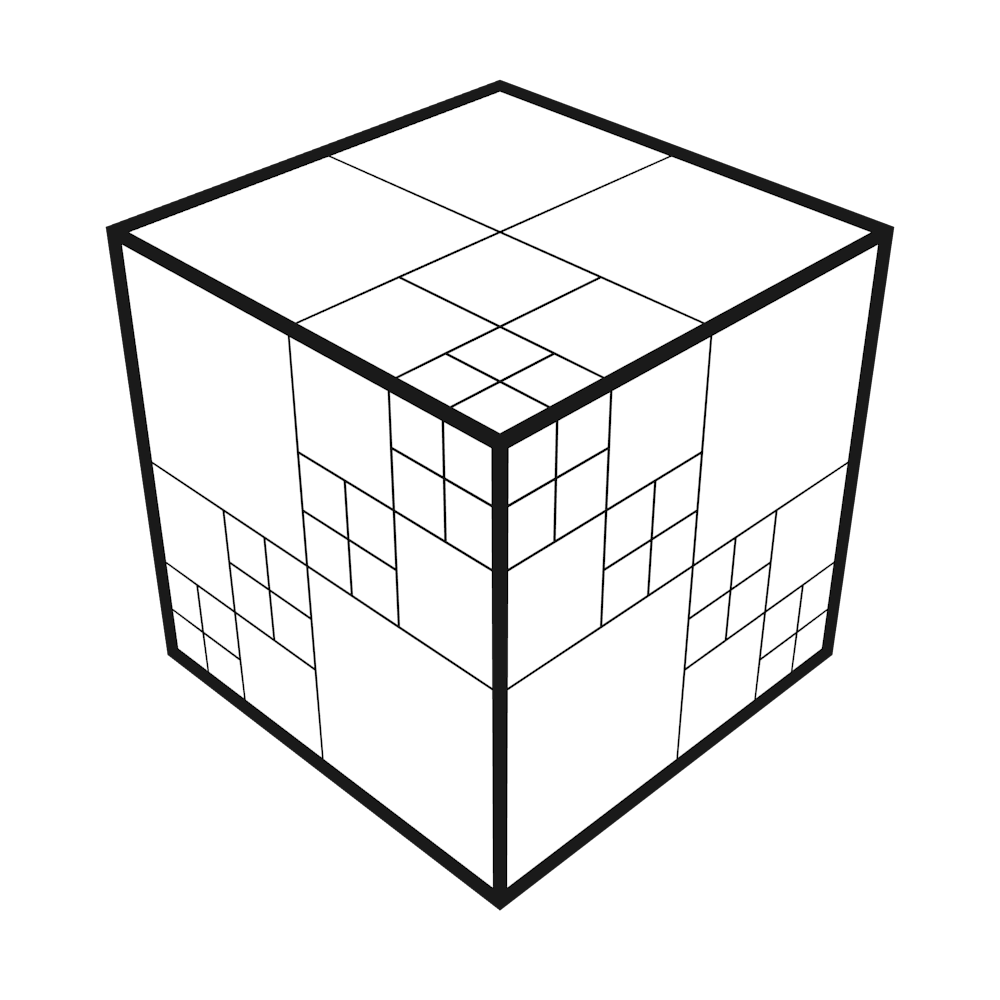
\includegraphics[width=6.5cm]{./img/raw/hs-datastructuren-overzicht/octree.png}};
    
\node at (4cm, -2.cm) {$\vdots$};
\node at (4cm, -10.5cm) {$\vdots$};




\node[inner sep=0pt] (level_0) at (4.0cm,-3cm  - 1.5cm)
    {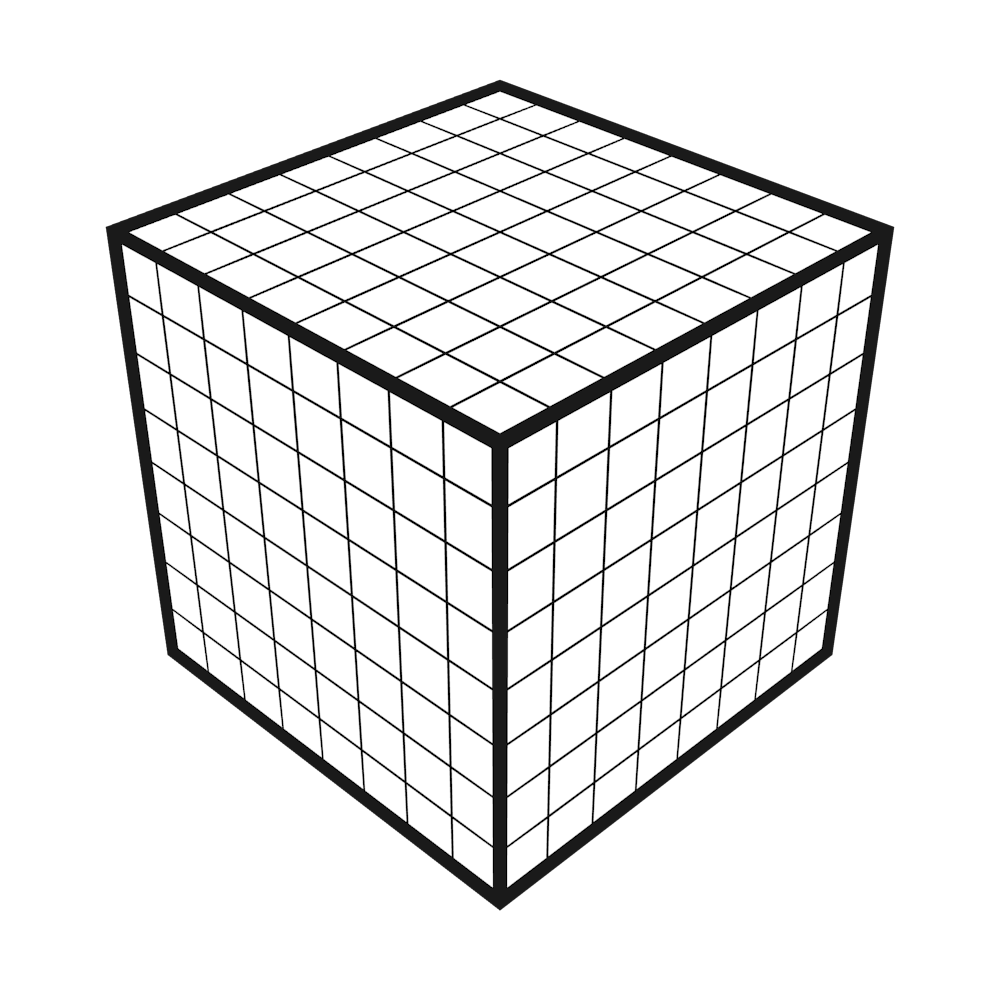
\includegraphics[width=3cm]{./img/raw/hs-datastructuren-overzicht/img1.png}};
\node[inner sep=0pt] (level_0) at (6.25cm,-2.75cm  - 1.5cm)
    {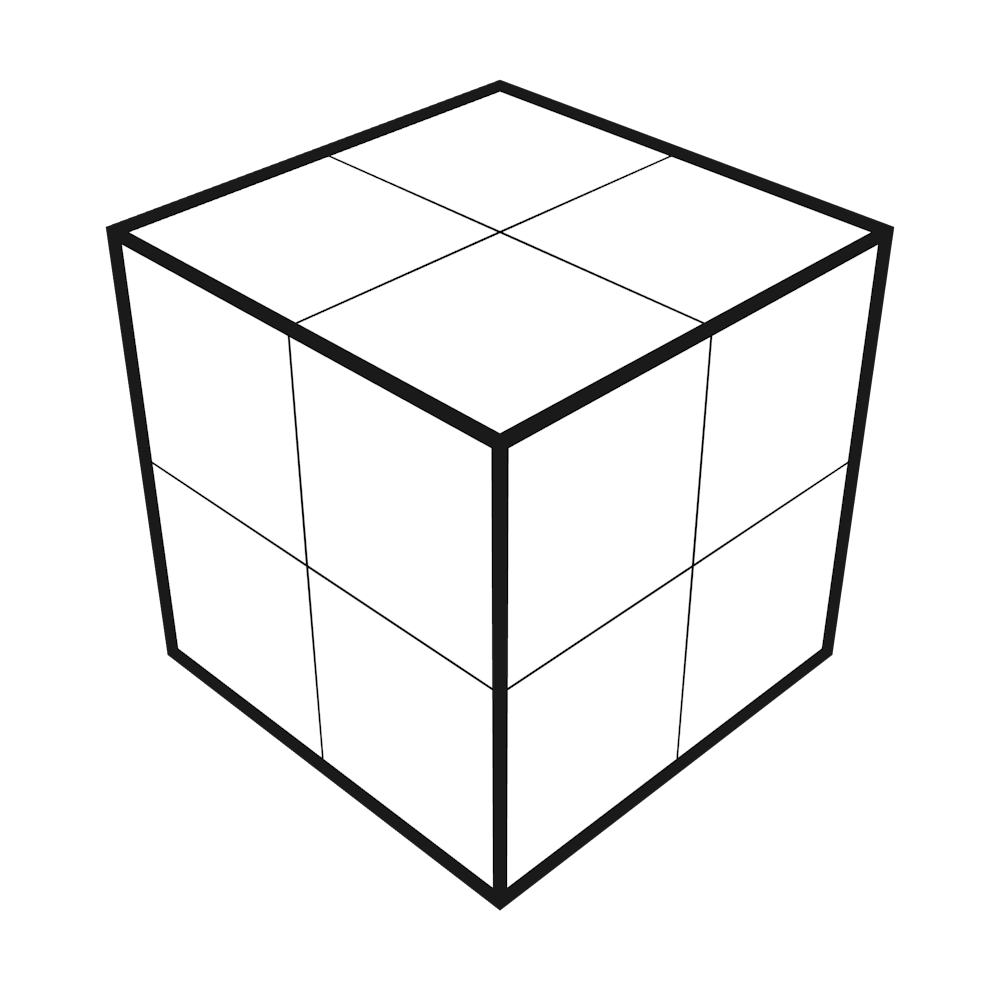
\includegraphics[width=2cm]{./img/raw/hs-datastructuren-overzicht/img2.png}};
\node[inner sep=0pt] (level_0) at (8.5cm,-3cm  - 1.5cm)
    {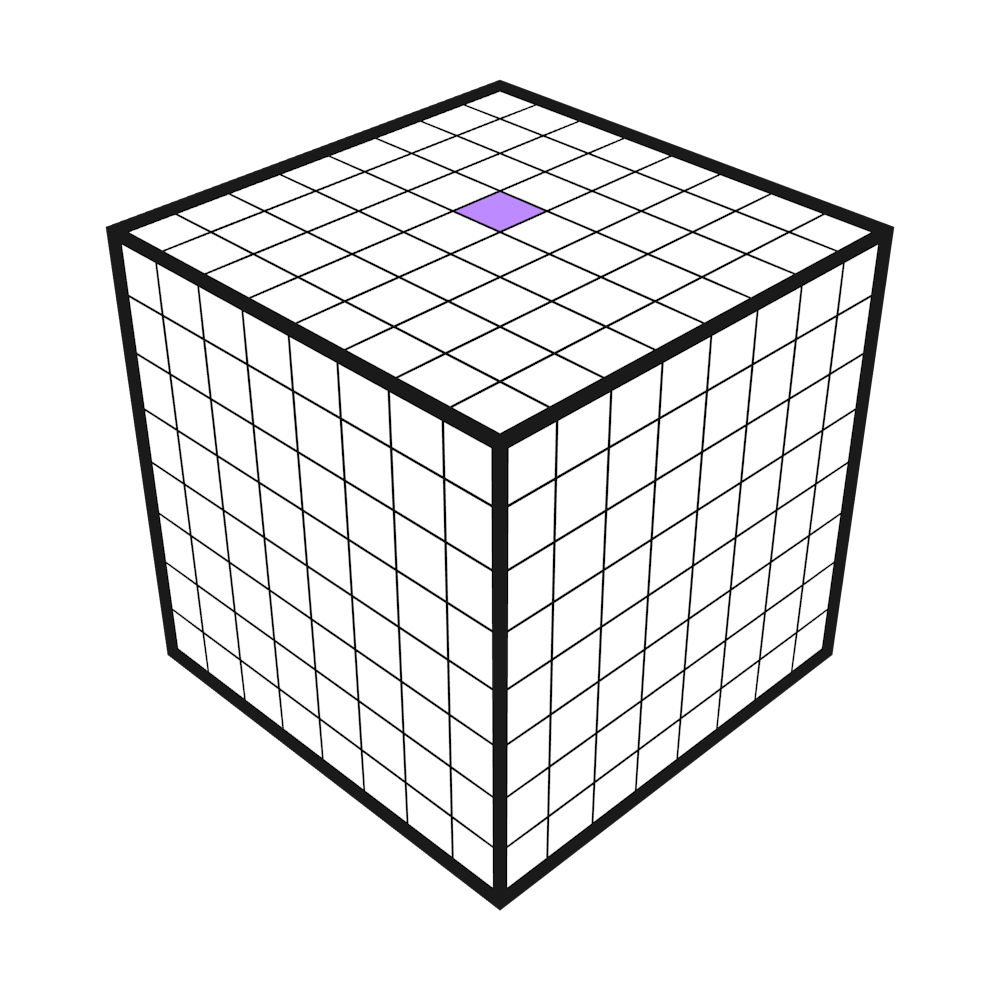
\includegraphics[width=3cm]{./img/raw/hs-datastructuren-overzicht/img3.png}};
\node[inner sep=0pt] (level_0) at (10.75cm,-2.75cm  - 1.5cm)
    {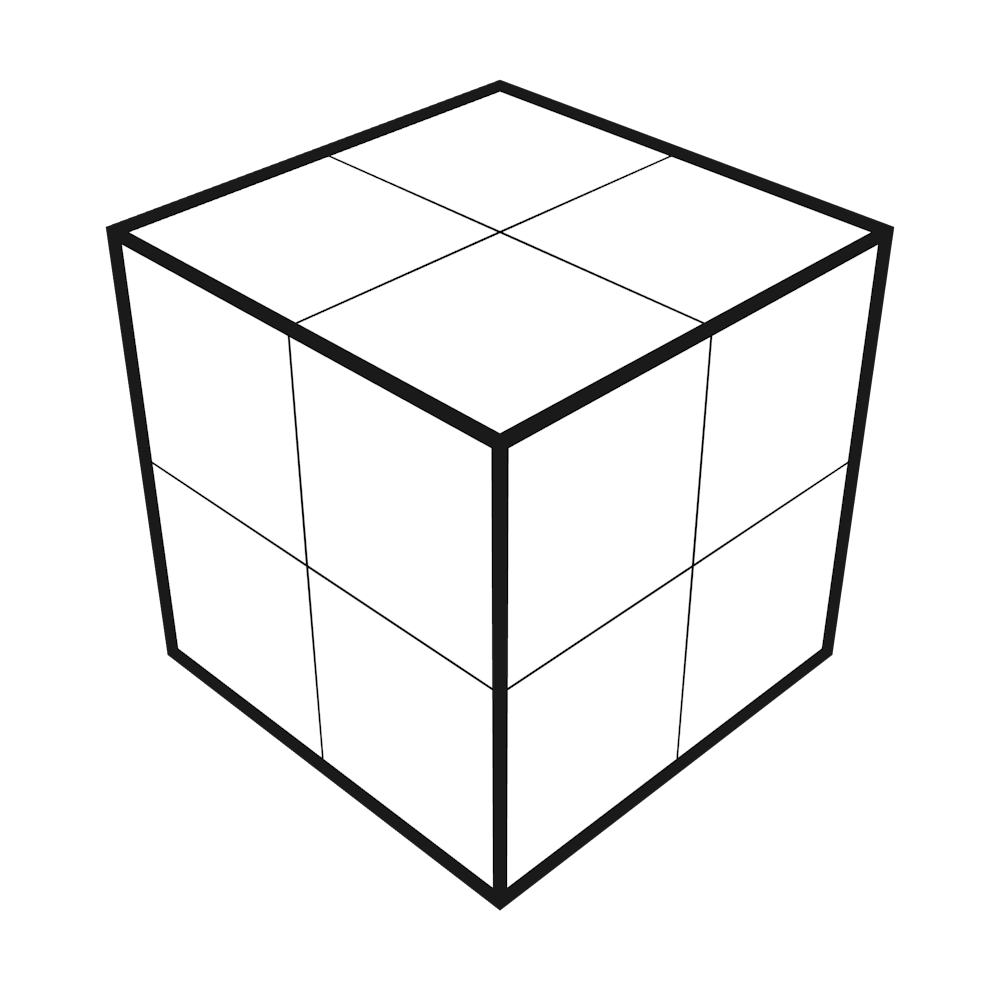
\includegraphics[width=2cm]{./img/raw/hs-datastructuren-overzicht/img2.png}};

\node[inner sep=0pt] (level_0) at (4.0cm,-3cm - 3.75cm  - 1.5cm)
    {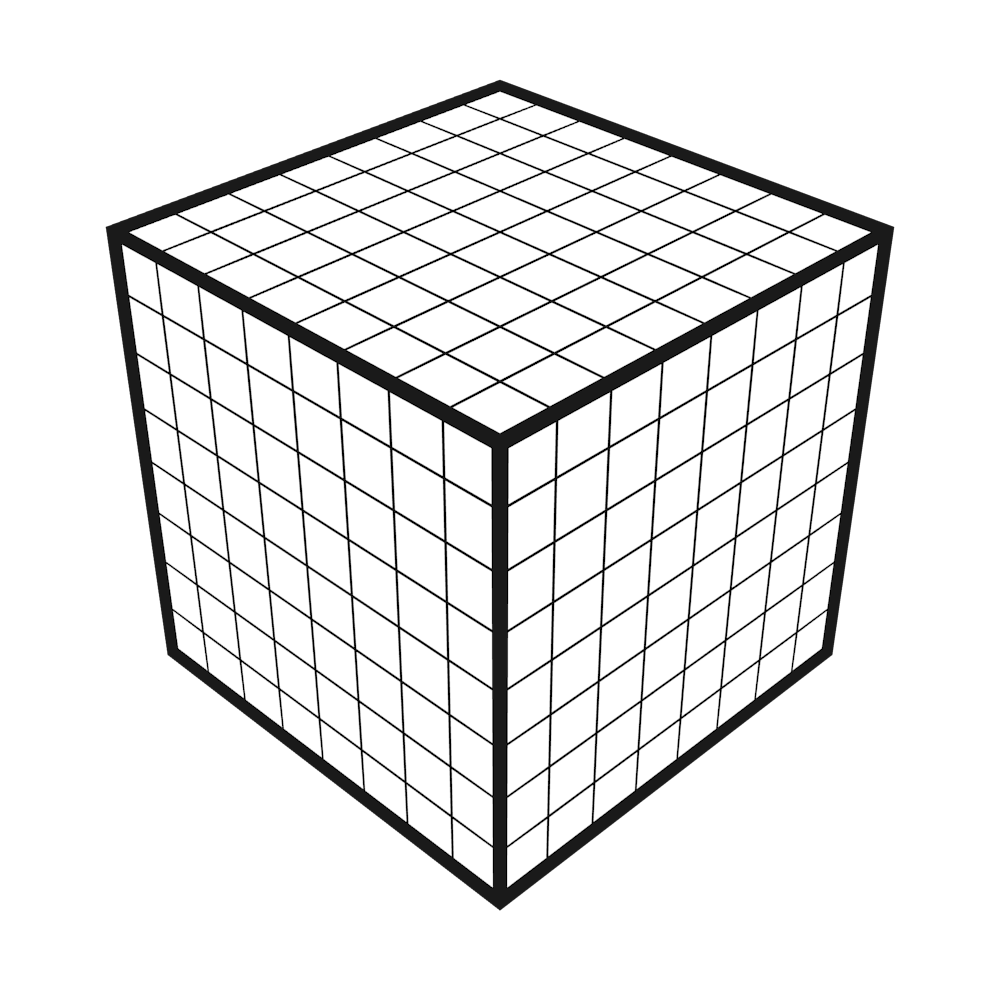
\includegraphics[width=3cm]{./img/raw/hs-datastructuren-overzicht/img1.png}};
\node[inner sep=0pt] (level_0) at (6.25cm,-2.75cm - 3.75cm  - 1.5cm)
    {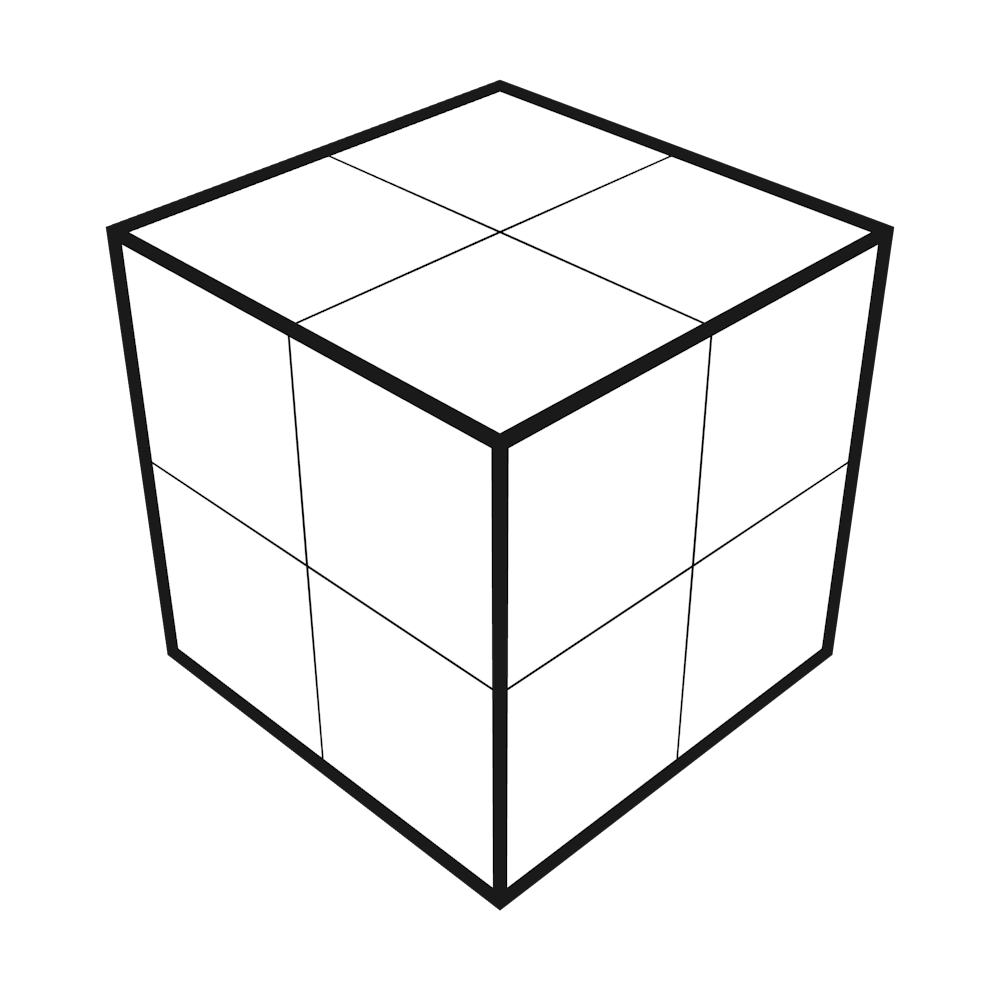
\includegraphics[width=2cm]{./img/raw/hs-datastructuren-overzicht/img2.png}};
\node[inner sep=0pt] (level_0) at (8.5cm,-3cm - 3.75cm  - 1.5cm)
    {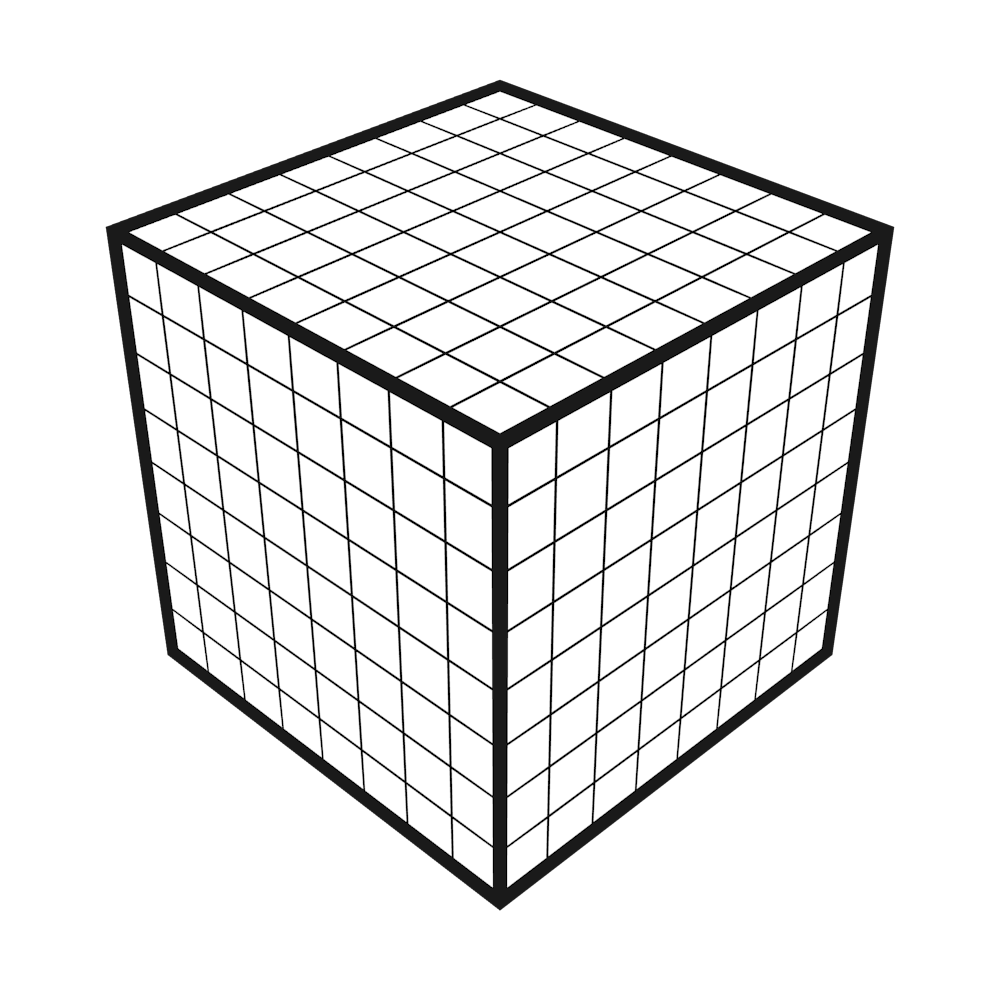
\includegraphics[width=3cm]{./img/raw/hs-datastructuren-overzicht/img1.png}};
\node[inner sep=0pt] (level_0) at (10.75cm,-2.75cm - 3.75cm  - 1.5cm)
    {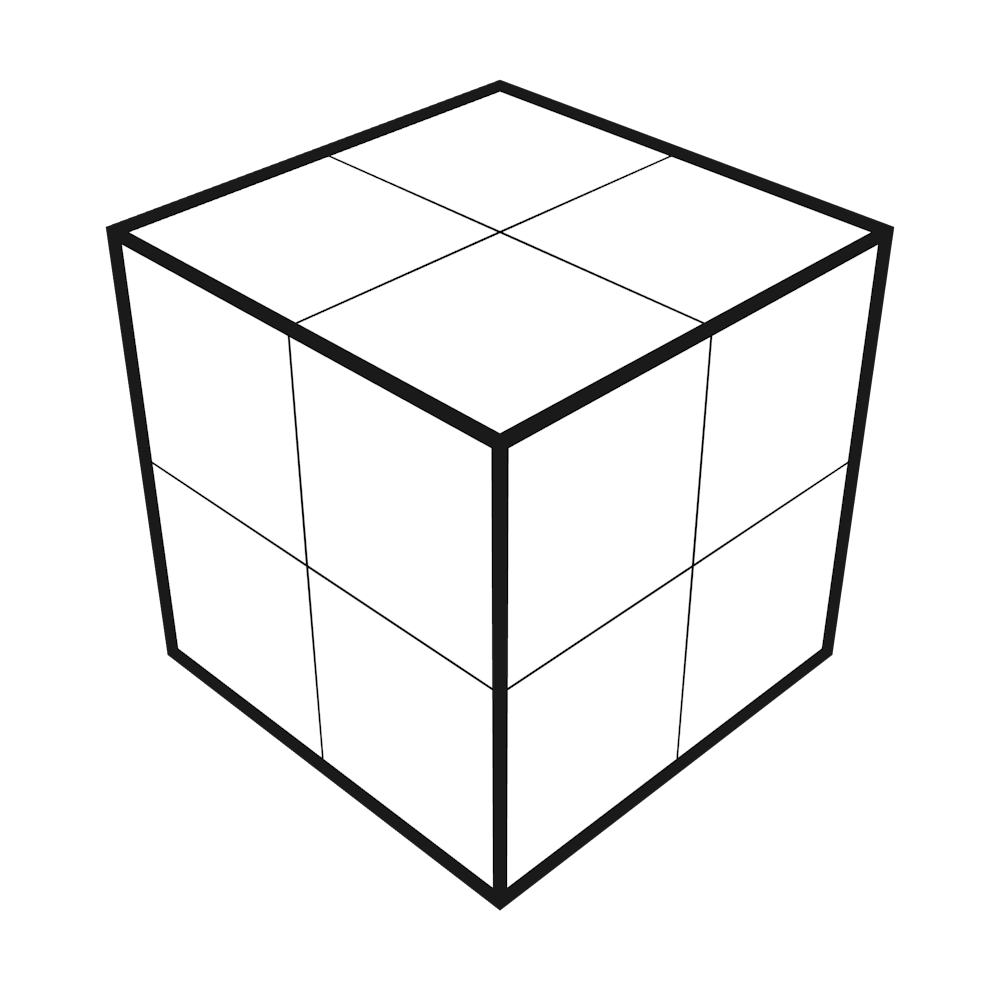
\includegraphics[width=2cm]{./img/raw/hs-datastructuren-overzicht/img2.png}};

\node at (11.75cm, -2.8cm) {\scriptsize layer $i$};
\node at (11.75cm, -2.8cm - 3.75cm) {\scriptsize layer $i + 1$};

\node at (3.0cm, -3.25cm) {$H_{1,i}$};
\node at (5.75cm, -3.25cm) {$\Phi_{1,i}$};
\node at (7.5cm, -3.25cm) {$H_{2,i}$};
\node at (10.25cm, -3.25cm) {$\Phi_{2,i}$};

\node at (3.0cm, -3.25cm -3.75cm) {$H_{1,i + 1}$};
\node at (5.75cm, -3.25cm  -3.75cm) {$\Phi_{1,i + 1}$};
\node at (7.5cm, -3.25cm -3.75cm) {$H_{2,i + 1}$};
\node at (10.25cm, -3.25cm -3.75cm) {$\Phi_{2,i + 1}$};

\node at (2cm, -2.5cm) (l1) {};
\node at (12.75cm, -2.5cm) (l2) {};
\draw[-, gray, very thin] (l1) -- (l2);

\node at (2cm, -2.5cm  -3.75cm) (l1) {};
\node at (12.75cm, -2.5cm  -3.75cm) (l2) {};
\draw[-, gray, very thin] (l1) -- (l2);

\node at (2cm, -2.5cm  -3.75cm -3.75cm) (l1) {};
\node at (12.75cm, -2.5cm  -3.75cm -3.75cm) (l2) {};
\draw[-, gray, very thin] (l1) -- (l2);

\node at (8.35cm, -3.63cm) (l1) {};
\node at (8.625cm, -3.63cm) (l2) {};

    \node at (-2.25cm + 10.75cm, -2cm + 1.5cm) (node_big) [grid_element_big, fill=tile0] {};
    \node at (-3.25cm + 10.75cm , -2cm + 1.5cm) (grid_l) [] {};
    \node at (-1.25cm + 10.75cm, -2cm + 1.5cm) (grid_r) [] {};
    \draw (grid_l.center) -- (grid_r.center);
    \node at (-2.25cm + 10.75cm, -1.5cm + 1.5cm) [] { \Large offset: $\mathit{k}$ };
    \node at (-2.25cm + 10.75cm, -2.5cm + 1.5cm) [] { \Large size: $\mathit{1}$ };

    \node at (-3.25cm + 10.75cm, -3cm + 1.55cm) (node_big_1) {};
    \node at (-1.25cm + 10.75cm, -3cm + 1.55cm) (node_big_2) {};


    \draw[gray] (node_big_1.center) -- (l1.center);
    \draw[gray] (node_big_2.center) -- (l2.center);
    
    \draw[-latex] (node_big.west) -- (light_index_0.south);


  \end{tikzpicture}
  \end{adjustbox}

  \caption{Overview of the data structures of Hashed Shading.}
  \label{fig:hs-data-structures}
\end{figure}


The goal of Hashed Shading is to improve the performance compared to Tiled and
Clustered Shading by reusing data structures between frames. The data structures
can be reused because the subdivision is independent from the view frustum. Thus
the data structures do not need to be rebuild when the camera position or
orientation changes. The subdivision of the scene space is done with an octree
representation such that it is both precise and memory efficient.

The following data structures are used within Hashed Shading:

\begin{itemize}
  \item Linkless Octree
  \item Light Index List
  \item Global Light List
\end{itemize}

\noindent These data structures are based on those of Tiled and Clustered
Shading. The Global Light List contains all the lights within the scene. The
Light Index List contains indices linking to the Global Light List. For each
leaf node the set of indices specifying the relevant lights is added to this
Light Index List. The set of relevant lights for each nonempty node within
the linkless octree can thus be specified with an offset and length marking
a subset within the Light Index List. This is illustrated in
figure \ref{fig:hs-data-structures}.

In order to construct these data structures the following steps need to be
executed

\begin{itemize}
  \item Define the subdivision of space.
  \item Calculate the influence of each light on this subdivision.
  \item Combine the influences into a single octree describing the whole scene.
  \item Construct the linkless octree and Light Index List based on the scene octree. 
\end{itemize}

\noindent The first step requires the origin and size of the octree to be set.
Once these values are specified it is possible to define the influence of each light.
The combination of all these influences leads to an octree representation of the
whole scene. In order to use this octree representation for light assignment, it needs
to be transformed into a linkless octree and a Light Index List. Once all these
steps have been completed, the constructed data structures can be used to speed up
the shading step of the rendering pipeline. Each of these steps will be explained
in more detail in the following sections.

% The goal of the Hashed Shading algorithm is to reduce the amount of work
% required to build the data structures between frames, in order to improve the
% overall performance compared to Tiled and Clustered Shading. It does so by
% dividing the scene space camera-independently. Thus the data structures can be
% reused between frames even if the camera position changes.
% The scene space is represented with an octree data structure. This representation
% is both precise and memory efficient.

% The used data structures are based on the data structured used within Tiled and
% Clustered Shading:

% \begin{itemize}
%   \item Linkless octree
%   \item Light index list
%   \item Global light list
% \end{itemize}

% \noindent The linkless octree replaces the tiles and clusters in Tiled and Clustered
% Shading respectively. It contains two integers per filled node, one that defines the
% offset within the light index list, and one that defines the size of the set of
% indices within the light index list.

% In order to construct these data structures the following steps have to be executed:

% \begin{itemize}
%   \item Define the scene space subdivision.
%   \item Calculate the influence of each light on the subdivision.
%   \item Combine the influences into one single scene octree.
%   \item Construct the linkless octree and light index list based on the scene octree.
% \end{itemize}

% \noindent The first step requires the origin of the octree and the total size to be
% calculated. Once these values are specified it is possible to define the influence
% of each light in the scene. The combination of these influences leads to a scene
% octree which has to be represented as a linkless octree in order to be used
% effectively on the GPU. Finally for each sample the set of relevant lights is calculated
% by descending into the octree. These steps will be explained in more detail in the
% following chapters.

\subsection{Specification of the Octree}

\begin{figure}[t]
  \begin{adjustbox}{minipage=\textwidth, scale=0.5}
  \centering
  \begin{tikzpicture}
    \node[inner sep=0pt] (img1) at (0.0\textwidth, -0.0\textwidth)
         {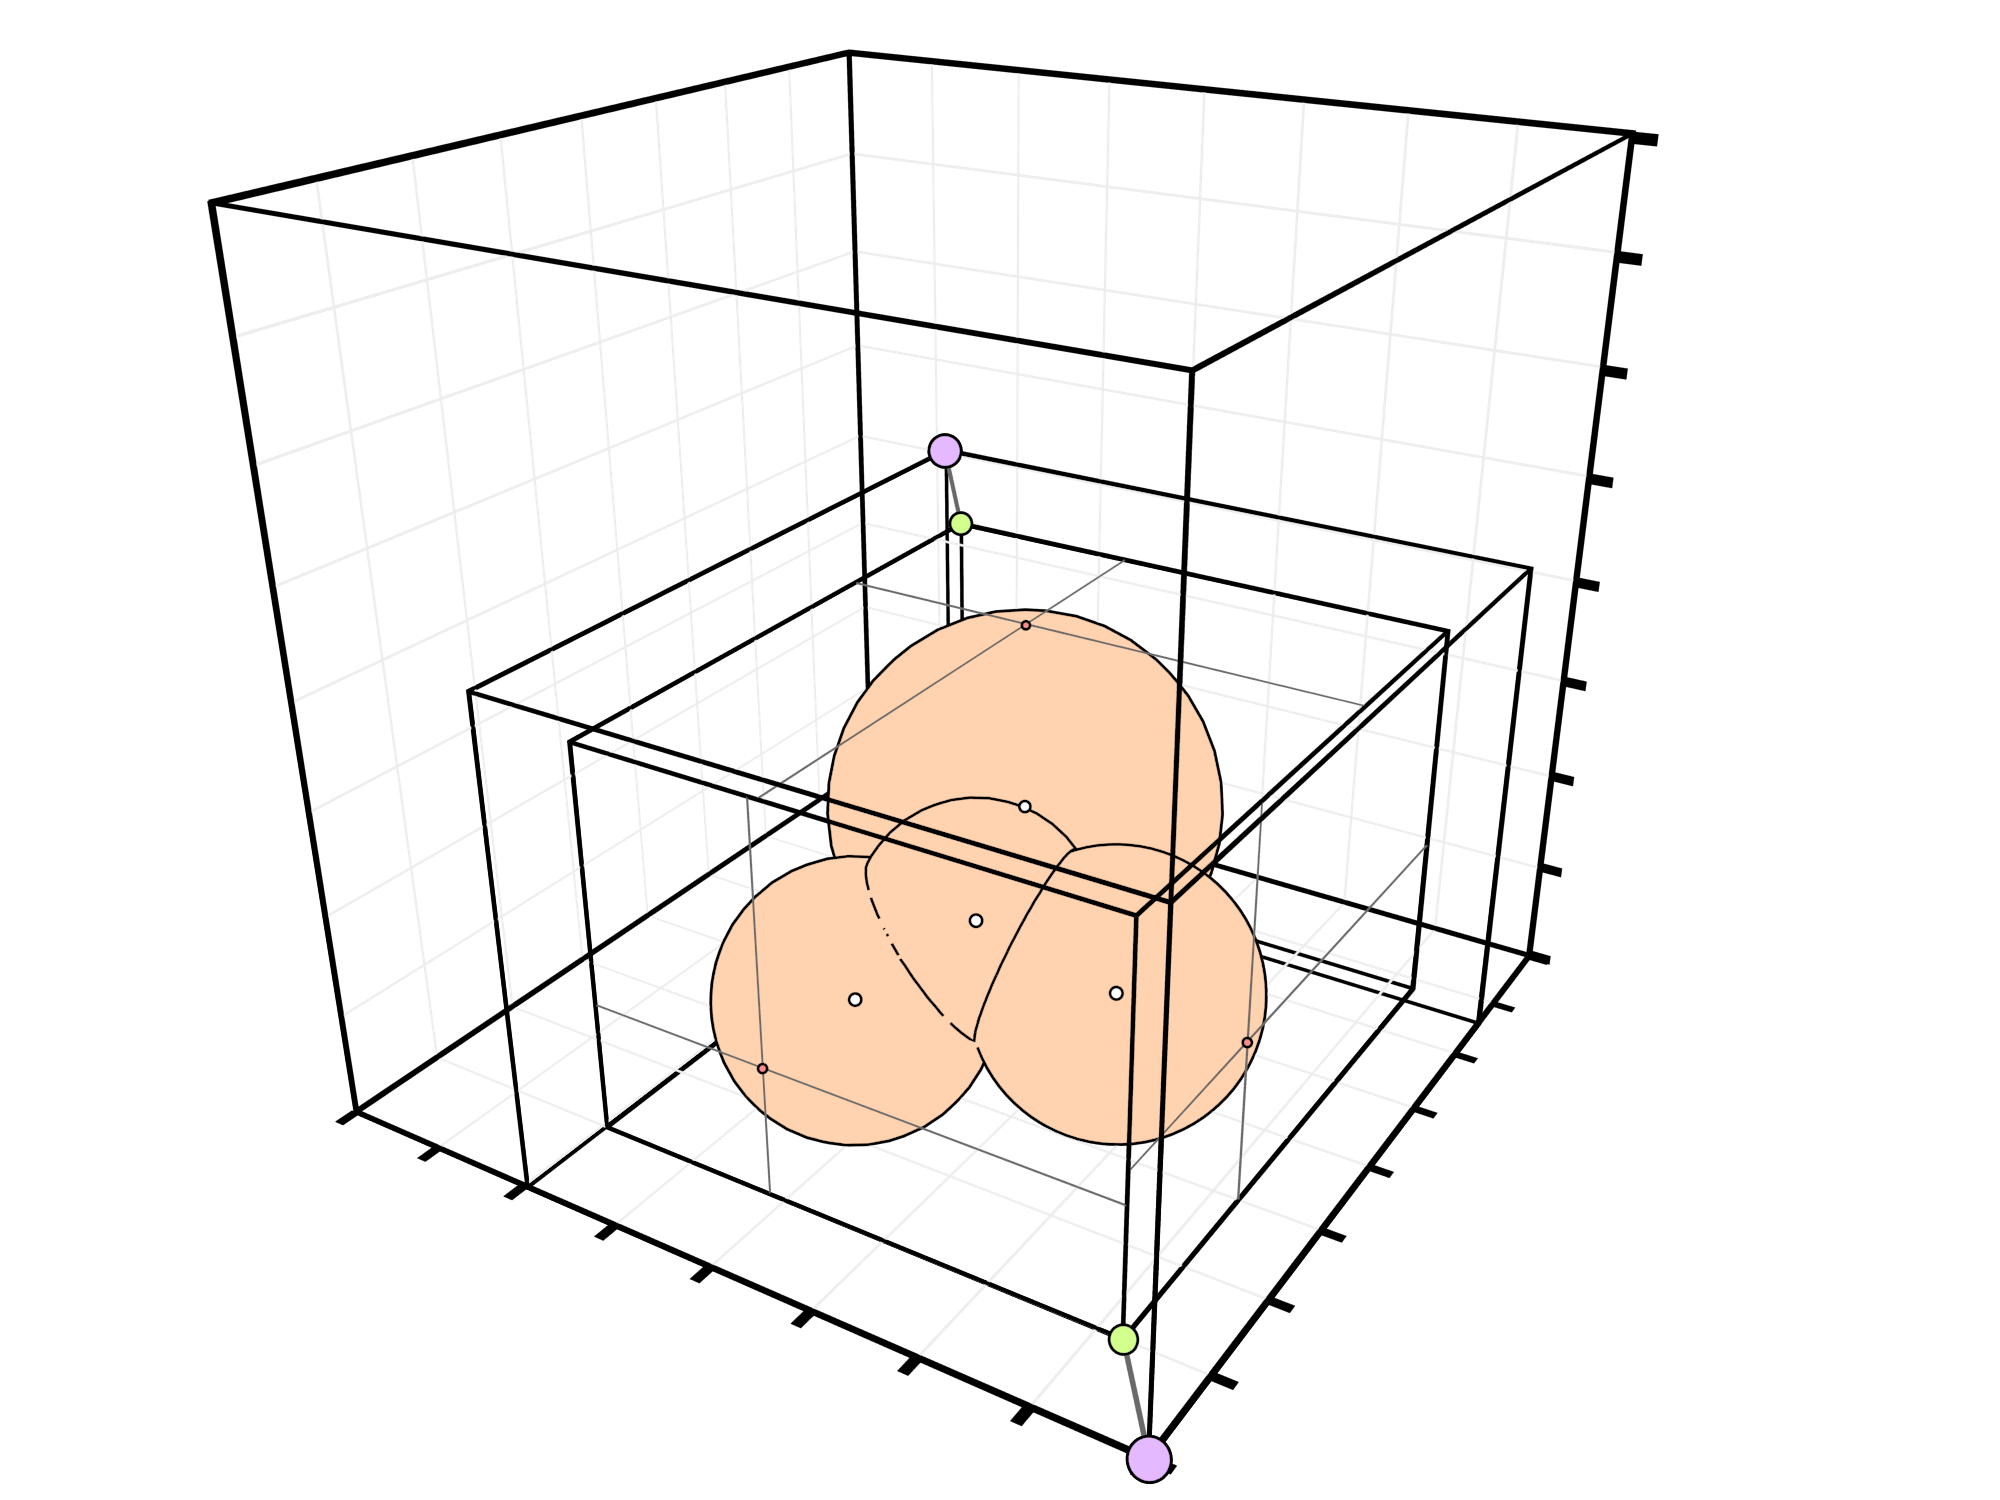
\includegraphics[width=12cm]{./img/raw/hs-opdeling-scene.png}};

    \node[] (camera-origin) at (0.225 * 16cm, -.08  * 16cm) {$2^l$};
    \node[] (camera-origin) at (0.075 * 16cm, -.28 * 16cm) {$\mathcal{O}$};
    \node[] (camera-origin) at (0.015  * 16cm, -.23  * 16cm) {$\mathbf{p}_\text{min}$};
    \node[] (camera-origin) at (0.015  * 16cm, .13  * 16cm) {$\mathbf{p}_\text{max}$};
  \end{tikzpicture}
  \end{adjustbox}
  \caption{The subdivision of the scene.}
  \label{fig:hs-subdivision-scene}
\end{figure}



To construct the octree a minimum bounding box containing all samples generated
at any point during the simulation needs to be defined. The minimum and maximum point
that define the bounding box can either be set by the developer or be constructed based
on the light volumes.

In order to ensure no values are generated outside the bounding box due to rounding errors.
a small offset is added to the points.

Once the bounding box has been defined, the size of the octree can be calculated.
The developer is responsible for setting the size of the nodes in the deepest layer of
the octree. Based on this node size, $\mathit{l}_o$, the size of the octree can be calculated.
Assuming that $\mathit{d}_i$ is the length of the longest face of the bounding box, the
size of the octree $\mathit{l}_o$ can be defined for the smallest possible $k$ such that holds

\begin{equation*}
  \mathit{l}_o = \mathit{l}_n \cdot 2^k \geq \mathit{d}_i
\end{equation*}

\noindent where $k$ is the number of layers within the octree. This is illustrated in figure
\ref{fig:hs-subdivision-scene}. With the origin and size of the octree defined it is possible to assign the
lights to this subdivision.

% To construct the octree a minimum bounding box which will fit all the lights at any
% point in time during the simulation, needs to be defined. The minimum and maximum
% points that define this bounding box can either be set by a developer or calculated
% based on the light volumes. In order to ensure small rounding errors do not affect
% the octree, an offset is added to these points.

% Once the bounding box has been defined the size of the octree can be calculated. The
% developer is responsible for setting the size of the nodes in the deepest layer of
% the octree. Based on this node size $\mathit{l}$, the size of the octree can be calculated.
% Assuming that $\mathit{d}_i$ is the maximum length of any of the sides of the
% bounding box, the number of layers is equal to the smallest value of $k$ for
% which holds

% \begin{equation*}
%   \mathit{l} \cdot 2^k \geq \mathit{d}_i
% \end{equation*}

% \noindent The size of the octree is equal to $\mathit{l} \cdot 2^k$.
% With the origin and size defined it is possible to assign the lights to this subdivision of
% space.

\subsection{Influence of Lights}

\begin{figure}[t]
  \centering
  \begin{subfigure}[b]{.3\linewidth}
    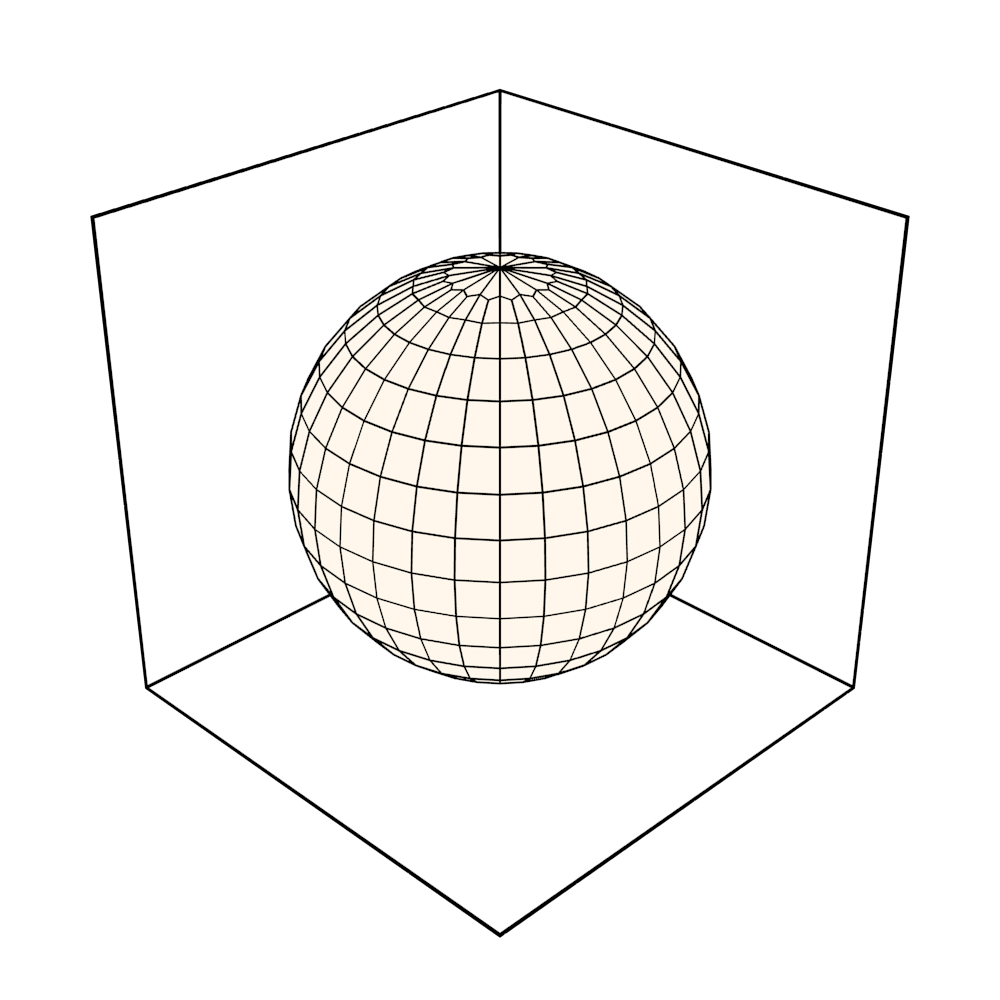
\includegraphics[width=\textwidth]{./img/raw/hs-slt-algorithm/hs-slt-algorithm-1.png}%
    \caption{\footnotesize Initial light volume}%
    \label{fig:hs-p1a}%
  \end{subfigure}
  %
  \begin{subfigure}[b]{.3\linewidth}
    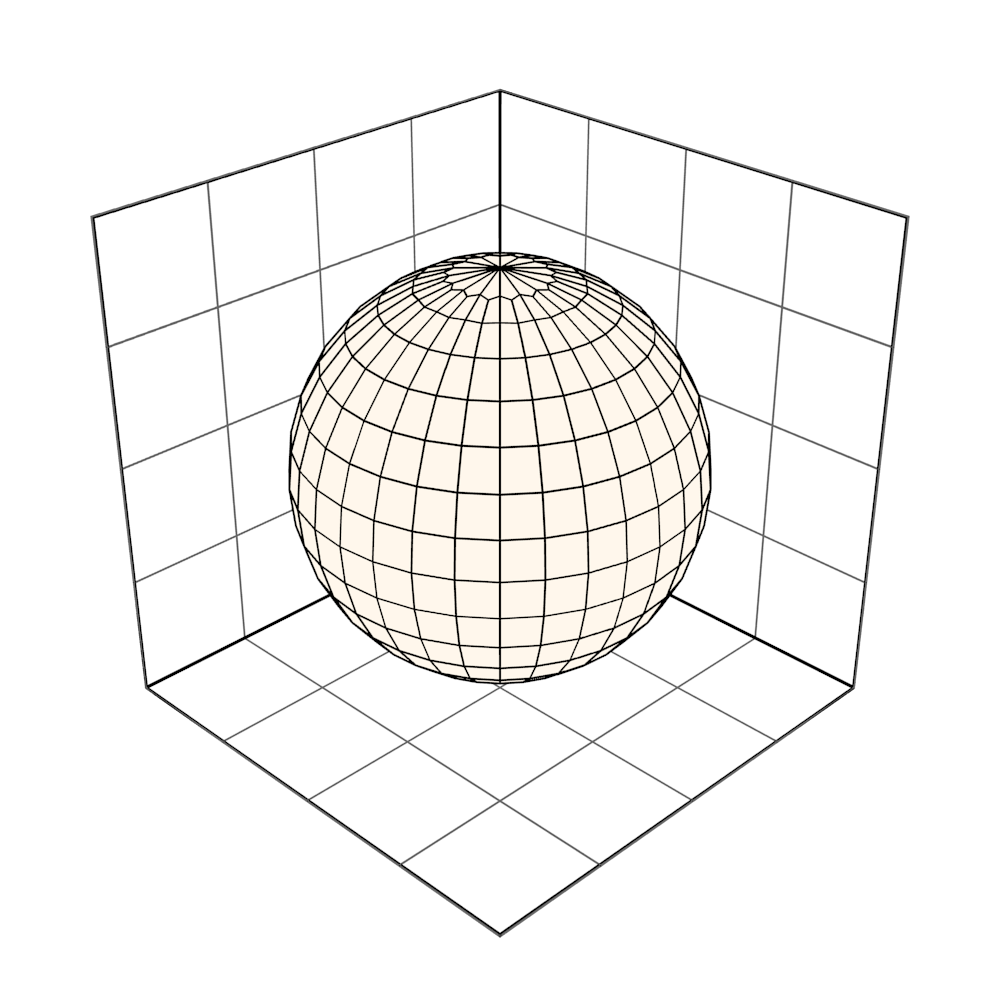
\includegraphics[width=\textwidth]{./img/raw/hs-slt-algorithm/hs-slt-algorithm-2.png}%
    \caption{\footnotesize Define grid}%
    \label{fig:hs-p1b}%
  \end{subfigure}
  %
  \begin{subfigure}[b]{.3\linewidth}
    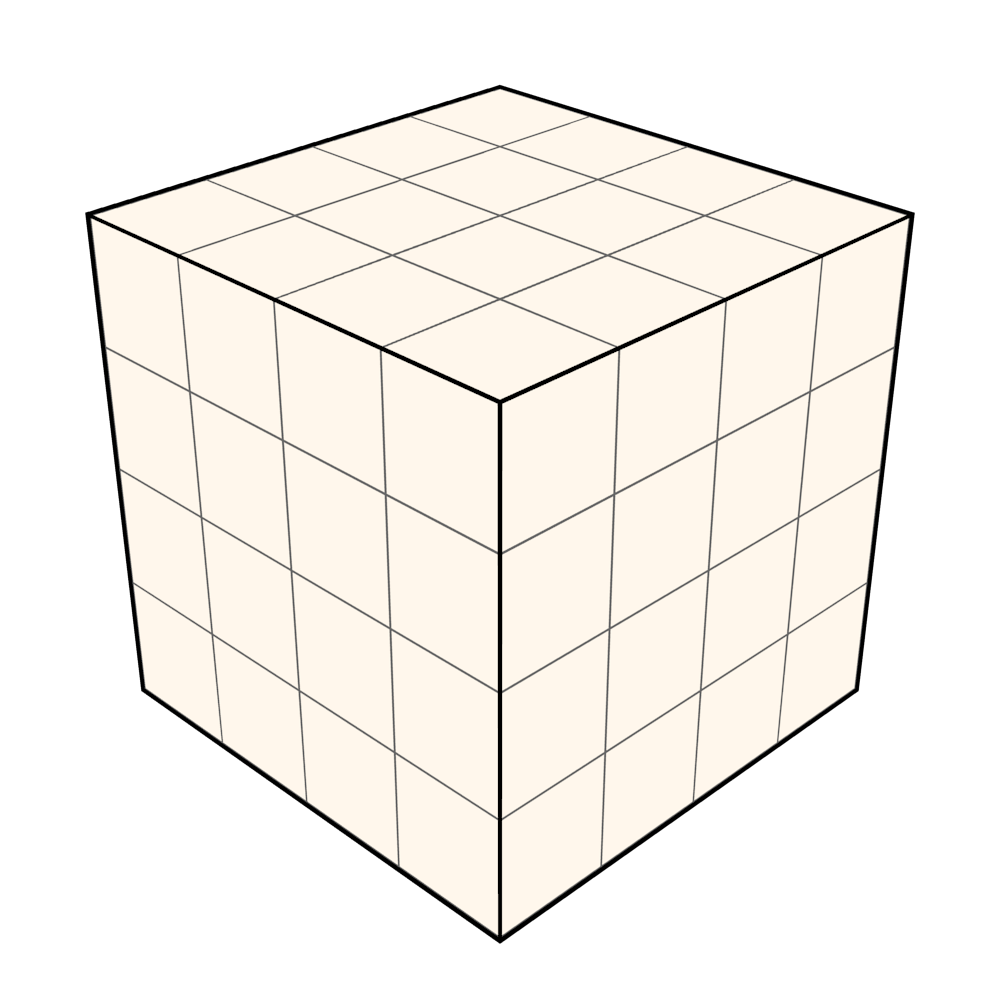
\includegraphics[width=\textwidth]{./img/raw/hs-slt-algorithm/hs-slt-algorithm-3.png}%
    \caption{\footnotesize Initialise grid}%
    \label{fig:hs-p1c}%
  \end{subfigure}
  \\
  \begin{subfigure}[b]{.3\linewidth}
    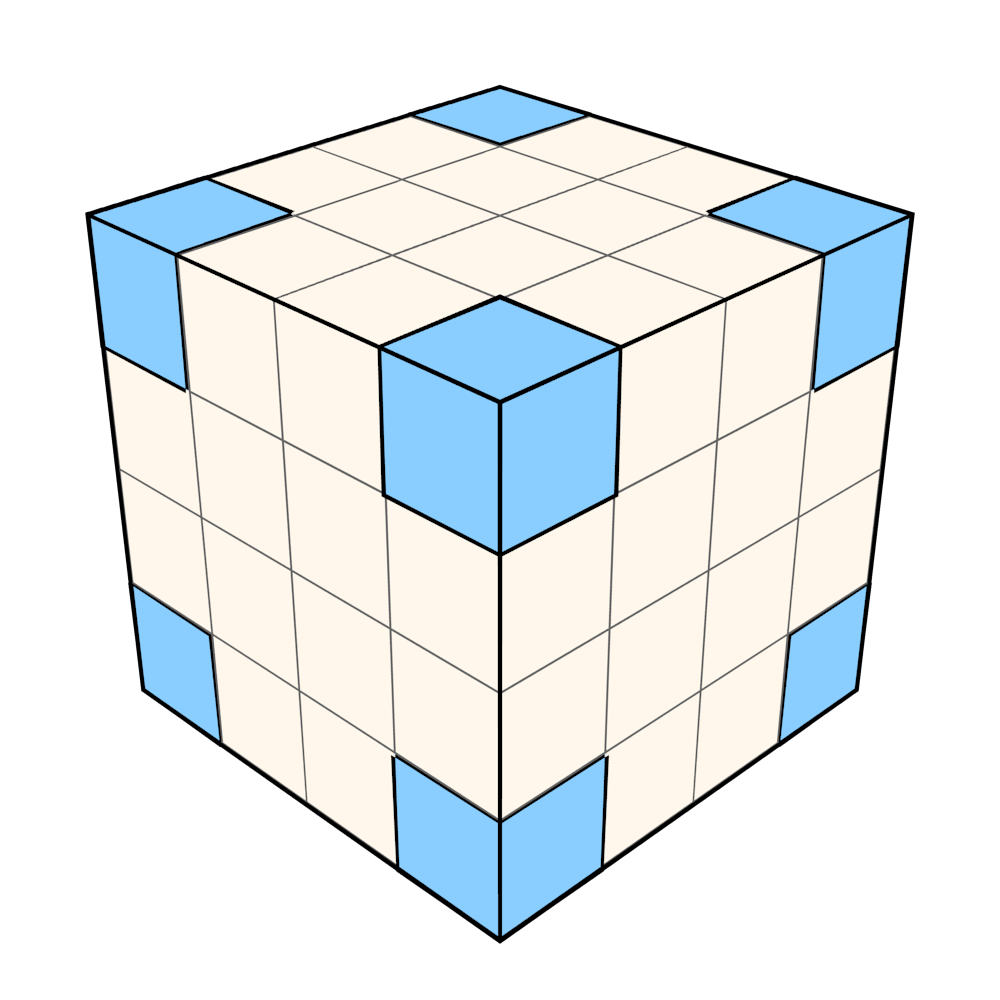
\includegraphics[width=\textwidth]{./img/raw/hs-slt-algorithm/hs-slt-algorithm-4.png}%
    \caption{\footnotesize Evaluate nodes}%
    \label{fig:hs-p1d}%
  \end{subfigure}
  %
  \begin{subfigure}[b]{.3\linewidth}
    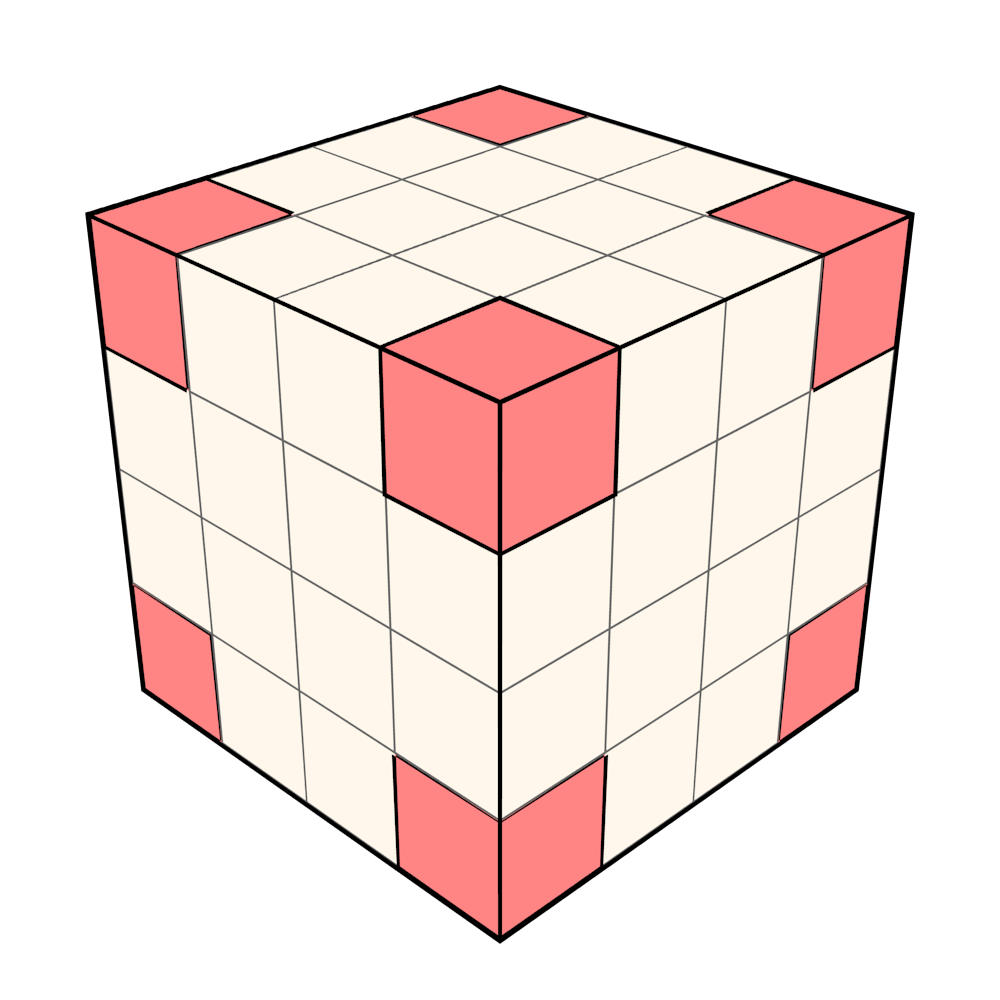
\includegraphics[width=\textwidth]{./img/raw/hs-slt-algorithm/hs-slt-algorithm-5.png}%
    \caption{\footnotesize Mark nodes}%
    \label{fig:hs-p1e}%
  \end{subfigure}
  %
  \begin{subfigure}[b]{.3\linewidth}
    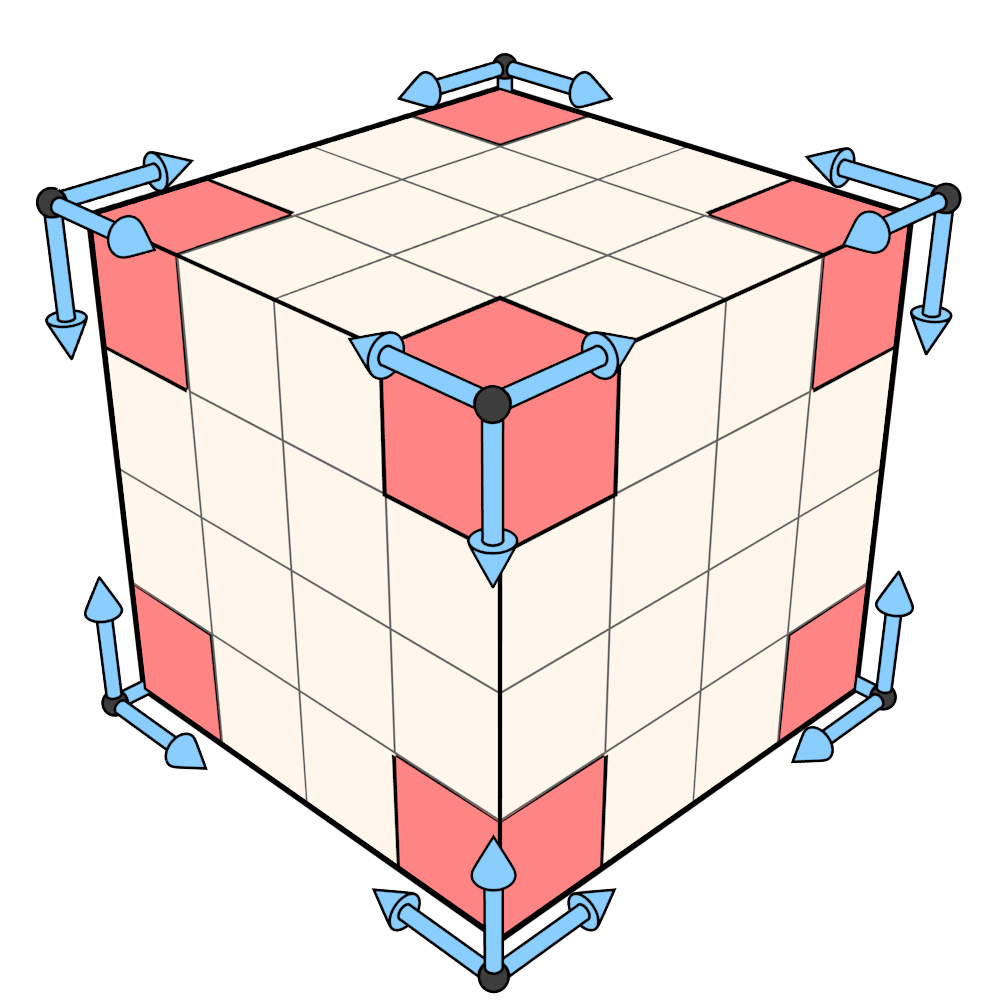
\includegraphics[width=\textwidth]{./img/raw/hs-slt-algorithm/hs-slt-algorithm-6.png}%
    \caption{\footnotesize Select nodes}%
    \label{fig:hs-p1f}%
  \end{subfigure}
  \\
  \begin{subfigure}[b]{.3\linewidth}
    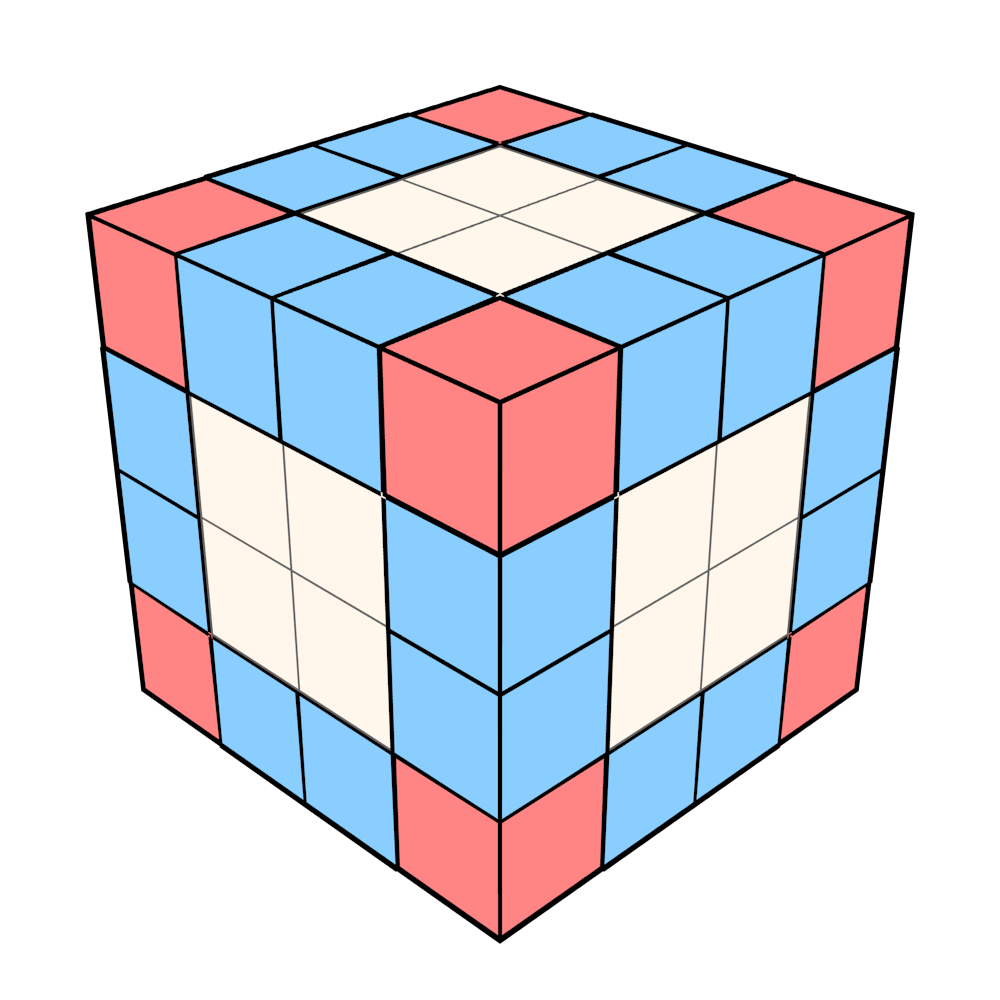
\includegraphics[width=\textwidth]{./img/raw/hs-slt-algorithm/hs-slt-algorithm-7.png}%
    \caption{\footnotesize Evaluate nodes}%
    \label{fig:hs-p1g}%
  \end{subfigure}
  %
  \begin{subfigure}[b]{.3\linewidth}
    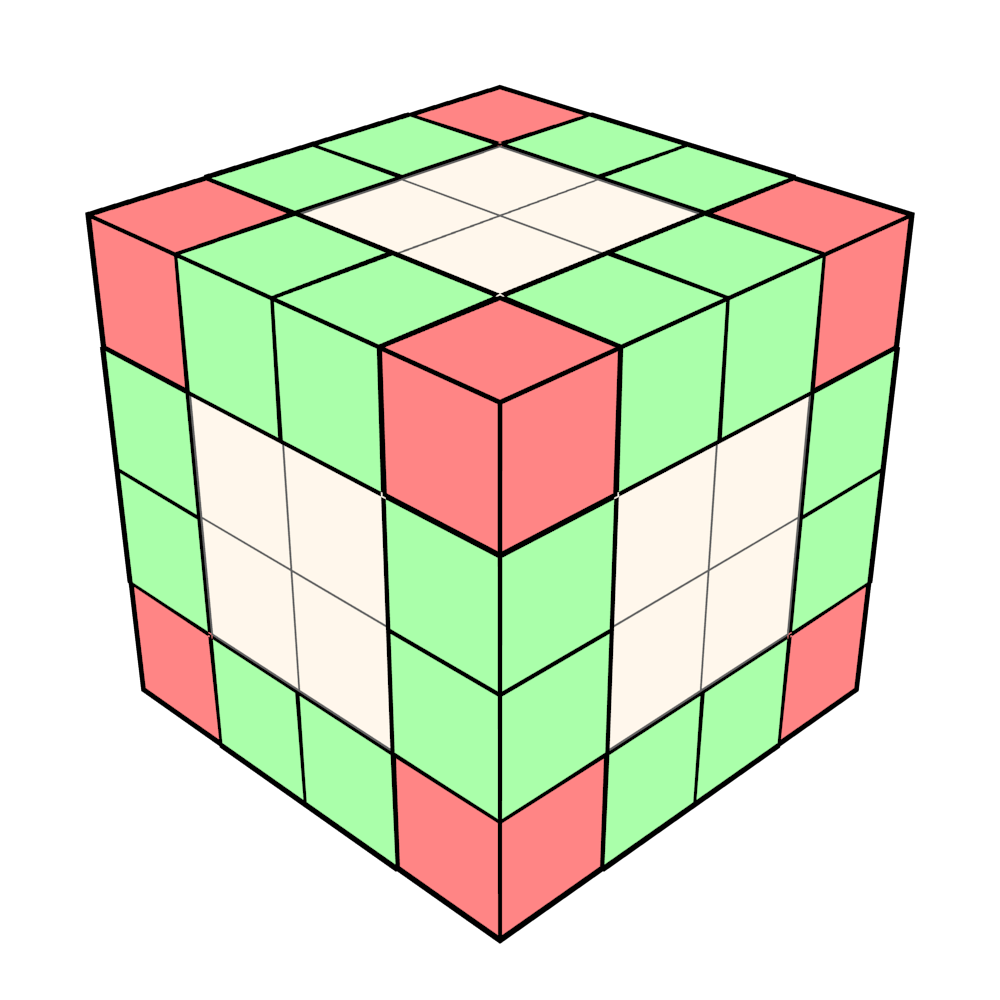
\includegraphics[width=\textwidth]{./img/raw/hs-slt-algorithm/hs-slt-algorithm-8.png}%
    \caption{\footnotesize Mark nodes}%
    \label{fig:hs-p1h}%
  \end{subfigure}
  %
  \begin{subfigure}[b]{.3\linewidth}
    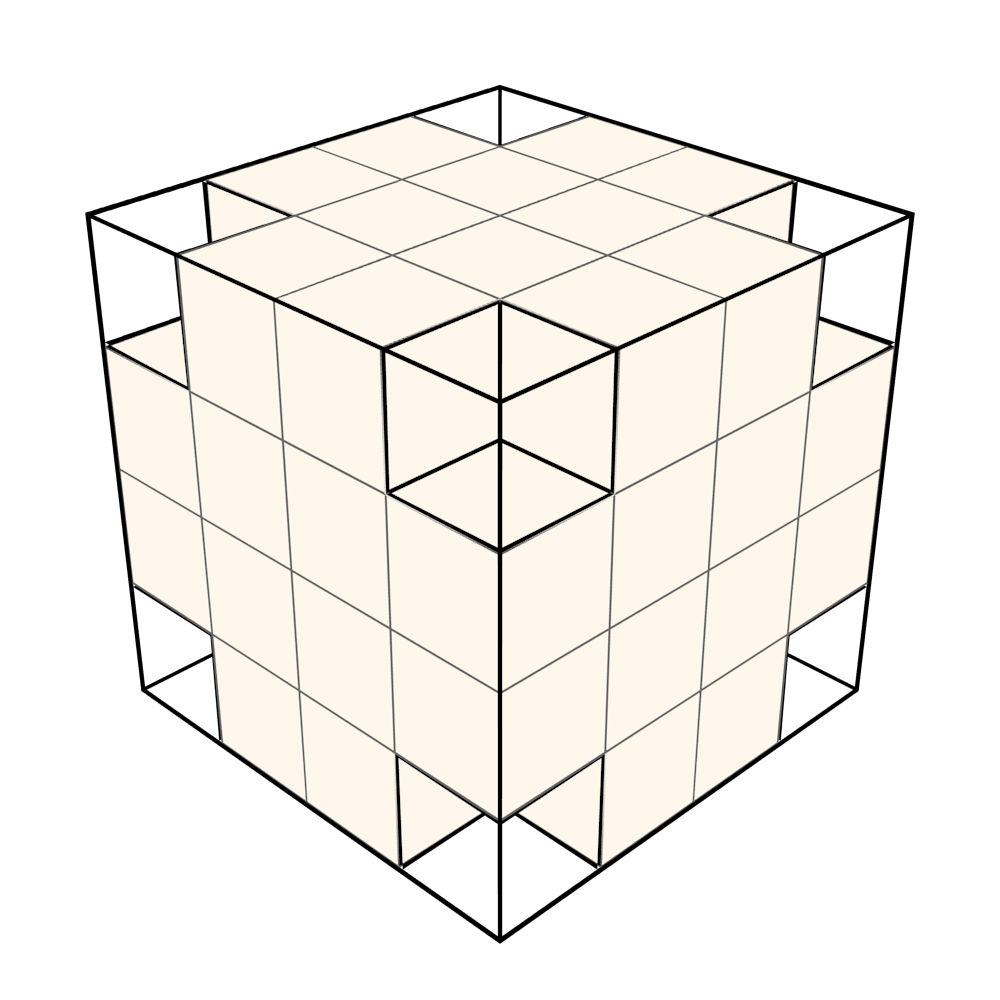
\includegraphics[width=\textwidth]{./img/raw/hs-slt-algorithm/hs-slt-algorithm-9.png}%
    \caption{\footnotesize Finalise grid}%
    \label{fig:hs-p1i}%
  \end{subfigure}

  \caption{Algorithm to determine the overlap of a single light with a grid of minimal nodes.}
  \label{fig:hs-p1}
\end{figure}


Within this paper only point lights are considered. Extending this algorithm to other
light types would require a similar approach to be drafted to assign the light volume
to the nodes with which it overlaps.

Any light has an influence on a node if the light volume overlaps with the node volume.
In the case of point lights whether a light overlaps with a node can be easily calculated
by comparing the distance between the light origin, $\mathbf{l}\mathtt{.orig}$, and the
point $\mathbf{p}$ within the node closest to the origin of the light, with the radius
$\mathbf{l}\mathtt{.radius}$ of the light. If this distance smaller than the radius,
then the node overlaps with the light:

\begin{equation*}
  \left\lVert \mathbf{p} - \mathbf{l}\mathtt{.orig} \right\rVert < \mathbf{l}\mathtt{.radius}
\end{equation*}

\noindent Point $\mathbf{p}$ within the node and closest to the origin of the light can be
easily calculated by clamping the dimensions of the light origin between the extreme values
of the node:

\begin{equation*}
   \mathbf{v} = \begin{pmatrix} \mathbf{l}.\mathtt{orig}_x \vert_{\mathbf{n}_{x}, \mathbf{n}_{x} + \mathit{l_n}} \\
                                \mathbf{l}.\mathtt{orig}_y \vert_{\mathbf{n}_{y}, \mathbf{n}_{y} + \mathit{l_n}} \\
                                \mathbf{l}.\mathtt{orig}_z \vert_{\mathbf{n}_{z}, \mathbf{n}_{z} + \mathit{l_n}} 
                \end{pmatrix} 
\end{equation*}

\noindent where $\mathbf{n}$ is the origin of the node.

This calculation does not need to be executed for each node within the whole space. Any node that
overlaps with a light volume falls within the minimal grid of nodes containing the whole light
volume. Furthermore, since each light volume is homogeneous, it is only necessary to establish the boundaries
of overlapping and non-overlapping nodes in order to know of all nodes whether they overlap.
This can be exploited by using a flood fill algorithm to reduce the amount of comparisons.
First, all nodes are assumed to be either overlapping or non-overlapping, then the nodes which
are not are marked as such. Since a sphere occupies slightly over half of its bounding box
volume and partially overlapping nodes are considered to be overlapping, all nodes within
the minimal grid, of nodes are initialised to be overlapping. Then starting from the corners
of the grid non-overlapping nodes are marked with a breadth first flood fill algorithm.
This process is illustrated in figure \ref{fig:hs-mark}.


Lastly, the way lights are represented in memory needs to be considered. In order to efficiently
calculate the change of dynamic lights the influence of lights in the previous frame can be compared
to the influence of lights in the current frame. In this case it is beneficial to save the
individual lights such that lights that actually change between frames can be evaluated
individually. The grid constructed in the previous step can be saved directly. In this case
each node requires a single bit in order to represent it. For small lights or large node sizes
this is a feasible approach. In case the lights are large or a small node size is used, this
approach could lead to a significant memory requirement. In these cases it is more beneficial
to represent the lights as an octree, to reduce the memory footprint. An example of such a
representation is given in figure \ref{fig:hs-slt}.

The octree representing a light can be efficiently constructed in a top-down fashion using the
constructed grid. First the octree node containing the whole grid is found. This node will
serve as the root node of the light octree. Then for each octree node the type is evaluated.
Initially there are three possible situations:

\begin{itemize}
  \item The octree node volume does not overlap with the grid.
  \item The octree node volume overlaps partly with the grid.
  \item The octree node volume falls within the grid.
\end{itemize}

\noindent In the first case the octree node is an empty leaf node, as no filled nodes lie outside
of the grid.

In the second case there are two possibilities. Either the node closest to the light origin
is empty, or it is nonempty. The octree node is respectively an empty leaf node or a branch node.
In the last case there are three possible situations. If the node closest to the light origin
is empty, then the octree node is empty as well. If this is not the case, then either the furthest
node from the light origin within the octree node is empty or nonempty. The octree node is
then respectively a branch node or a nonempty leaf node. In the case that an octree node is
a branch node, then the types of the children of this node are evaluated as well.

\begin{figure}
  \centering
  \begin{subfigure}[b]{.45\linewidth}
    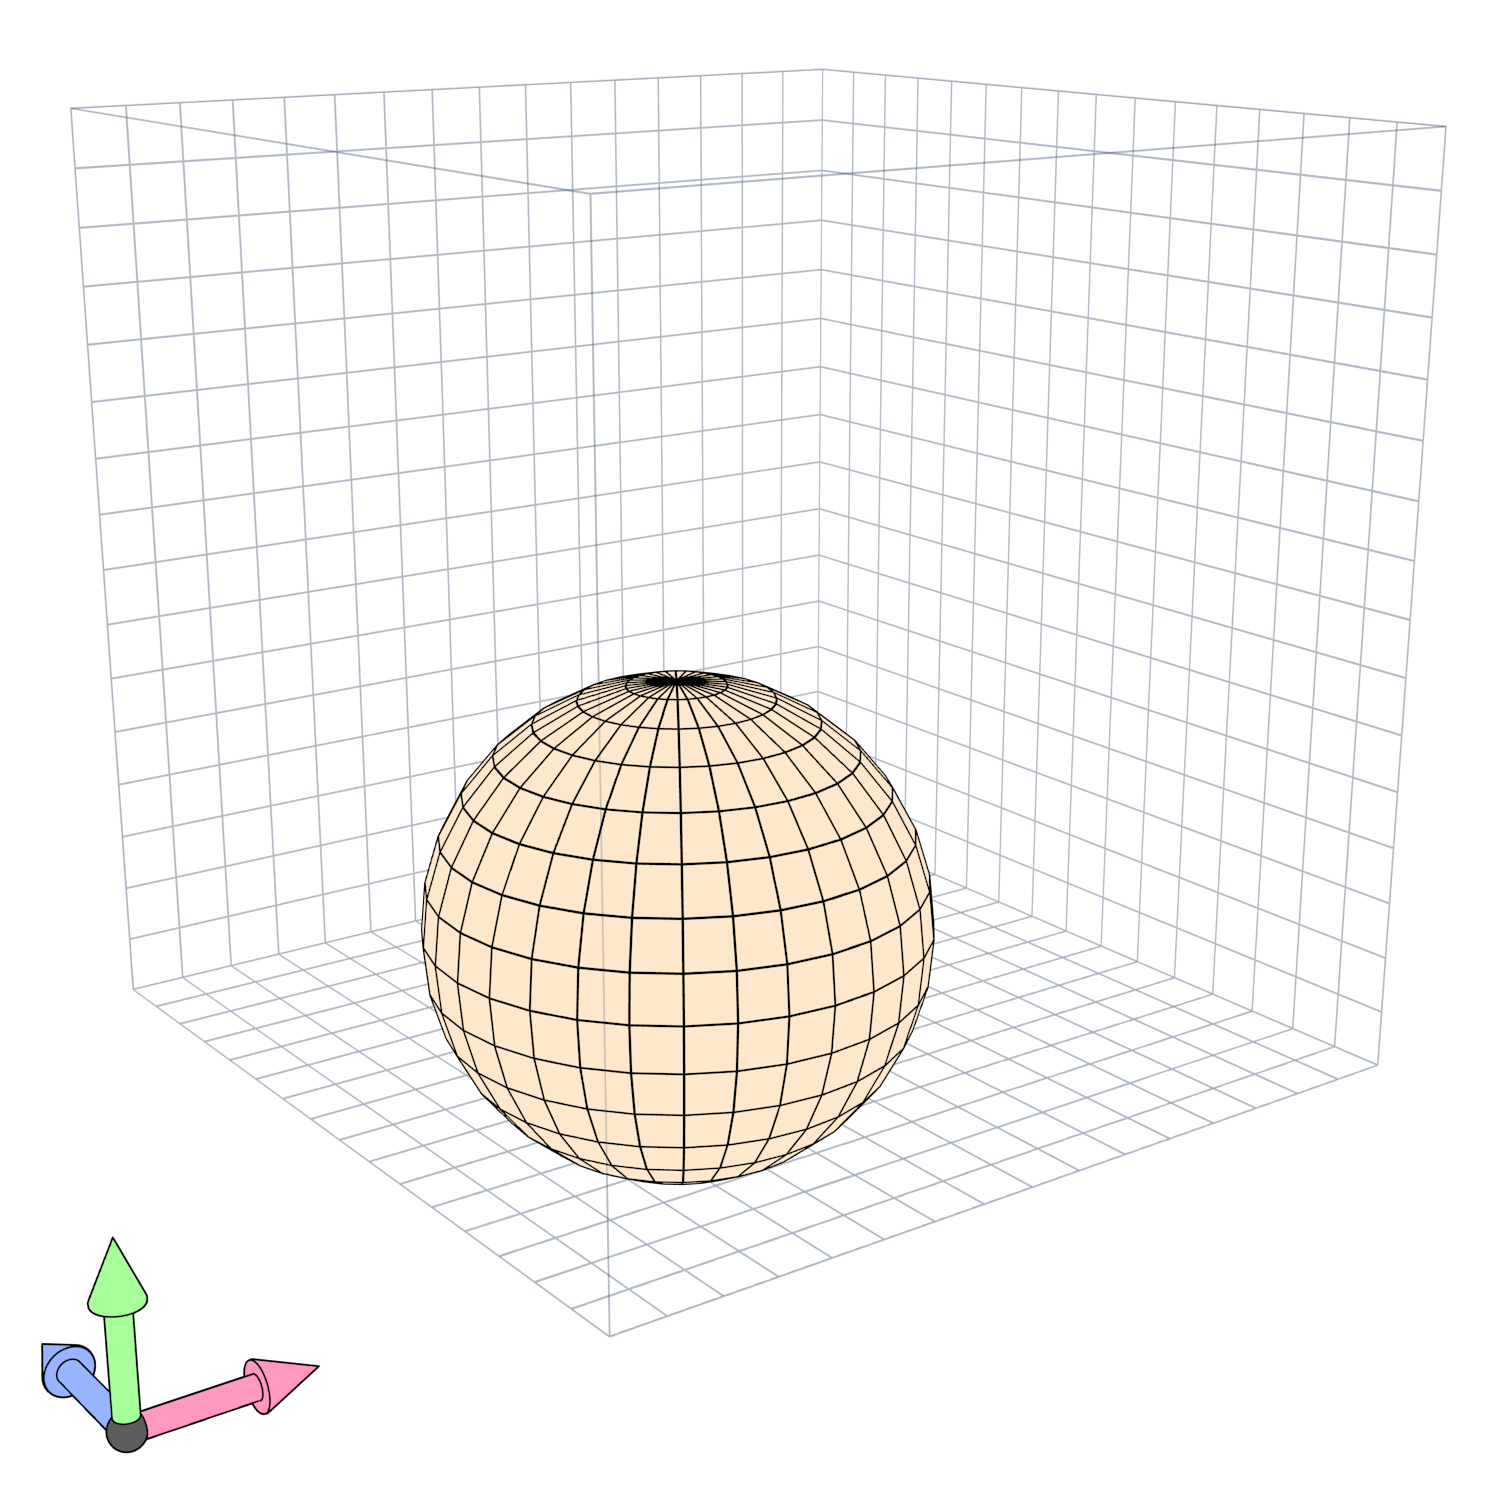
\includegraphics[width=\textwidth]{./img/raw/hs-slt/hs-slt_left.png}%
    \caption{Light volume}%
    \label{fig:hs-slt-left}%
  \end{subfigure} %
  \begin{subfigure}[b]{.45\linewidth}%
    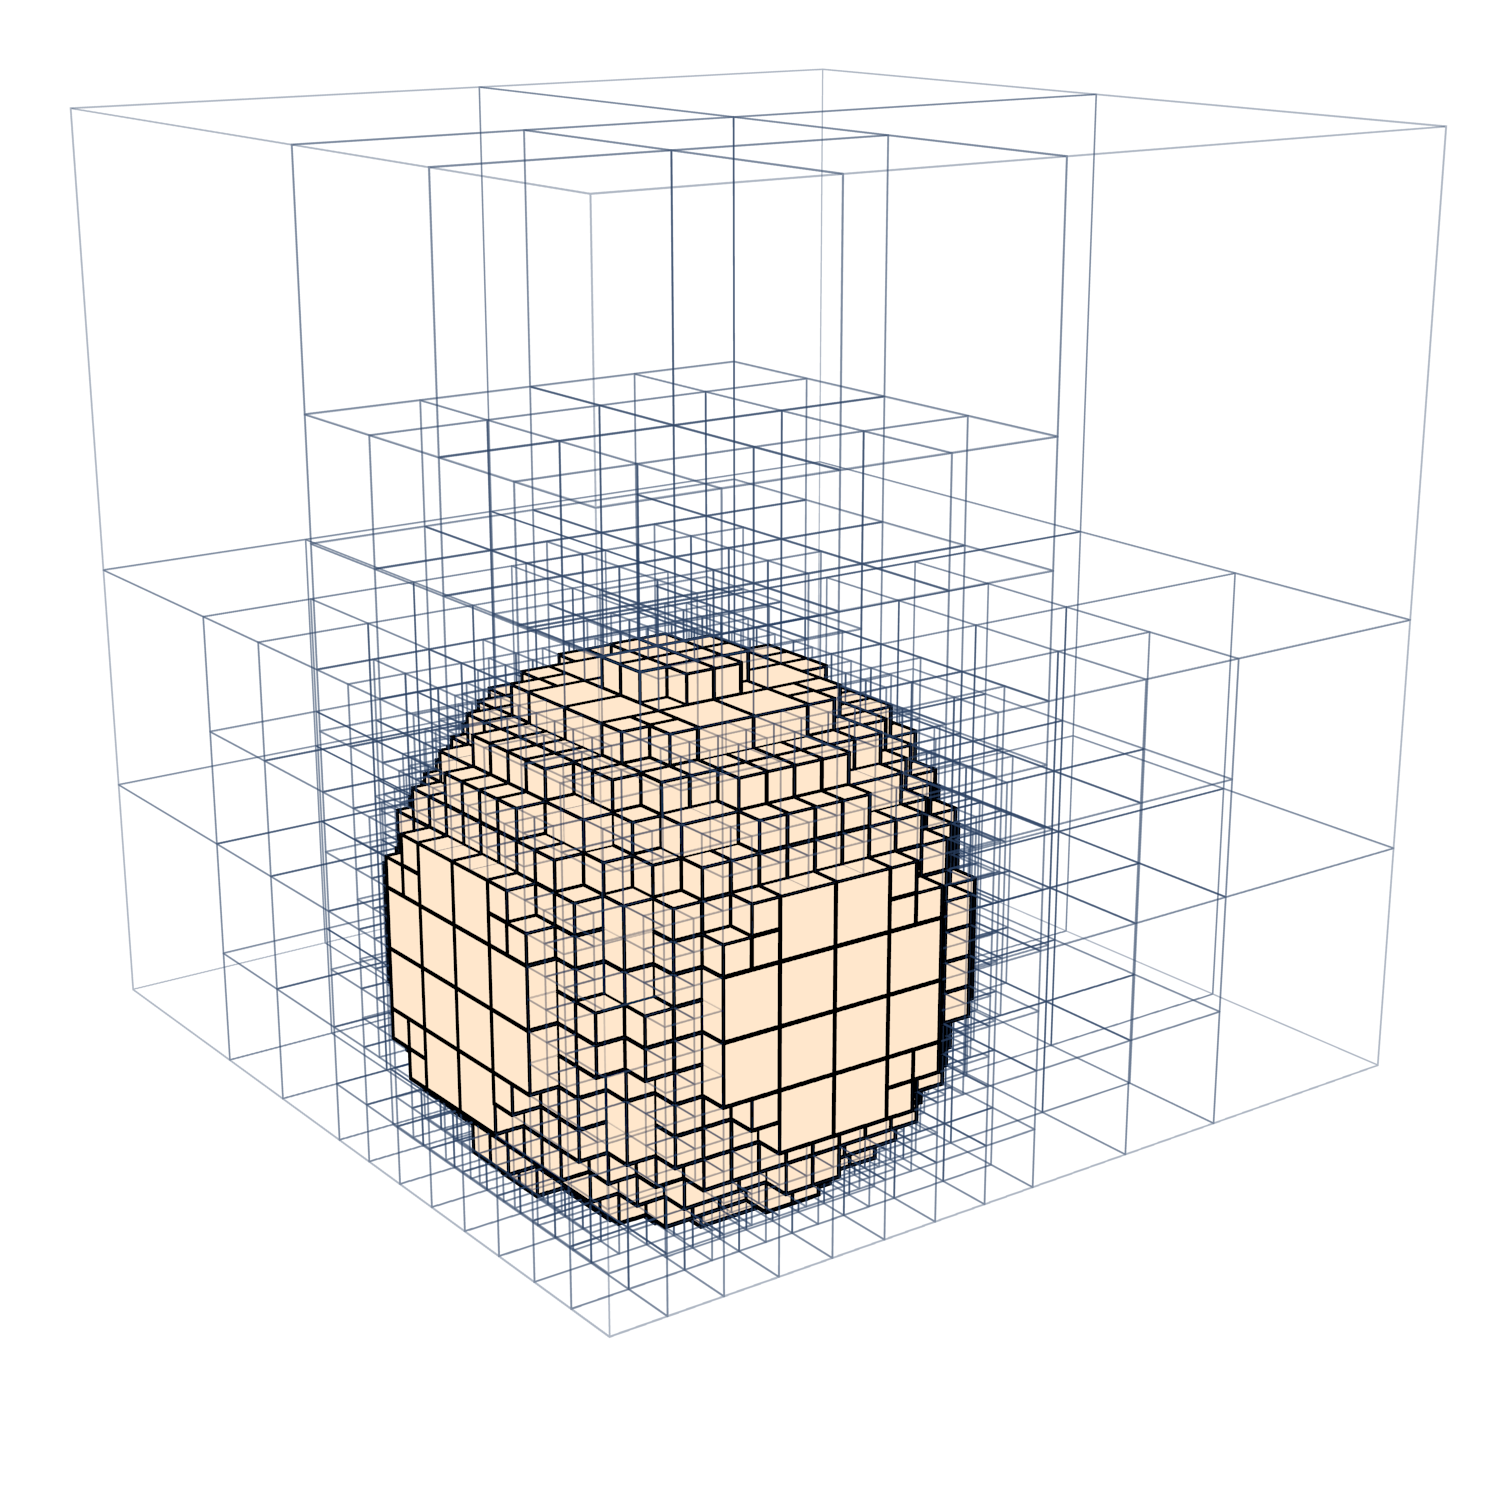
\includegraphics[width=\textwidth]{./img/raw/hs-slt/hs-slt_right.png}%
    \caption{Octree subdivision}%
    \label{fig:hs-slt-right}%
  \end{subfigure}
  \caption{Octree representation of a single light volume.}
  \label{fig:hs-slt}
\end{figure}


% We only consider point lights within the current implementation of the algorithm. In order to
% support different light types, a similar approach need to be developed for these lights, such
% that the influence they have on the scene space subdivision can be efficiently calculated.

% Any light has an influence on a node if the light volume overlaps with the node volume. In case
% of point lights this can be easily calculated by comparing the distance between the light origin
% $\mathbf{l}\mathtt{.orig}$ and the point inside the node volume closest to the light origin $\mathbf{p}$,
% and the radius of the point light $\mathbf{l}\mathtt{.radius}$
% volume. In case this distance is smaller than the radius, the node volume overlaps with the light
% volume:

% \begin{equation*}
%   \left\lVert \mathbf{p} - \mathbf{l}\mathtt{.orig} \right\rVert < \mathbf{l}\mathtt{.radius}
% \end{equation*}

% \noindent Point $\mathbf{p}$ within the node volume and closest to the light origin can be easily
% calculated by clamping the light volume per dimension between the extreme values of the node:

% \begin{equation*}
%   \mathbf{v} = \begin{pmatrix} \mathbf{l}.\mathtt{orig}_x \vert_{\mathbf{n}_{x}, \mathbf{n}_{x} + \mathit{l}} \\
%                                \mathbf{l}.\mathtt{orig}_y \vert_{\mathbf{n}_{y}, \mathbf{n}_{y} + \mathit{l}} \\
%                                \mathbf{l}.\mathtt{orig}_z \vert_{\mathbf{n}_{z}, \mathbf{n}_{z} + \mathit{l}} 
% \end{pmatrix} 
% \end{equation*}

% \noindent where $\mathbf{n}$ is the origin of the node.

% This calculation does not need to be executed for every node within the scene space.
% Any node overlapping with the light lies within the minimal grid of nodes which contains the light volume.
% Furthermore, each light is uniform, meaning that once we have established the boundaries of overlapping
% and non-overlapping nodes, we know of all nodes whether they are overlapping or not.
% This can be exploited by using a flood-fill algorithm to either fill the empty or overlapping nodes.

% Because the volume of a sphere is slightly bigger than half its bounding box and because partly
% overlapping nodes are also considered non-empty, we start with the assumption that each node
% is overlapping, and fill the non-overlapping nodes. We use a breadth-first flood fill algorithm,
% where each of the corner nodes of the grid are the seed nodes. If a node overlaps it is marked as
% checked and removed from the queue. If a node does not overlap it is marked as checked and the
% three nodes adjacent to the node facing inwards are added to the queue if they have not been checked
% before. This is process is shown in figure \ref{}.
% Once the queue is empty, all overlapping nodes have been determined.

% \begin{figure}
  \centering
  \begin{subfigure}[b]{.45\linewidth}
    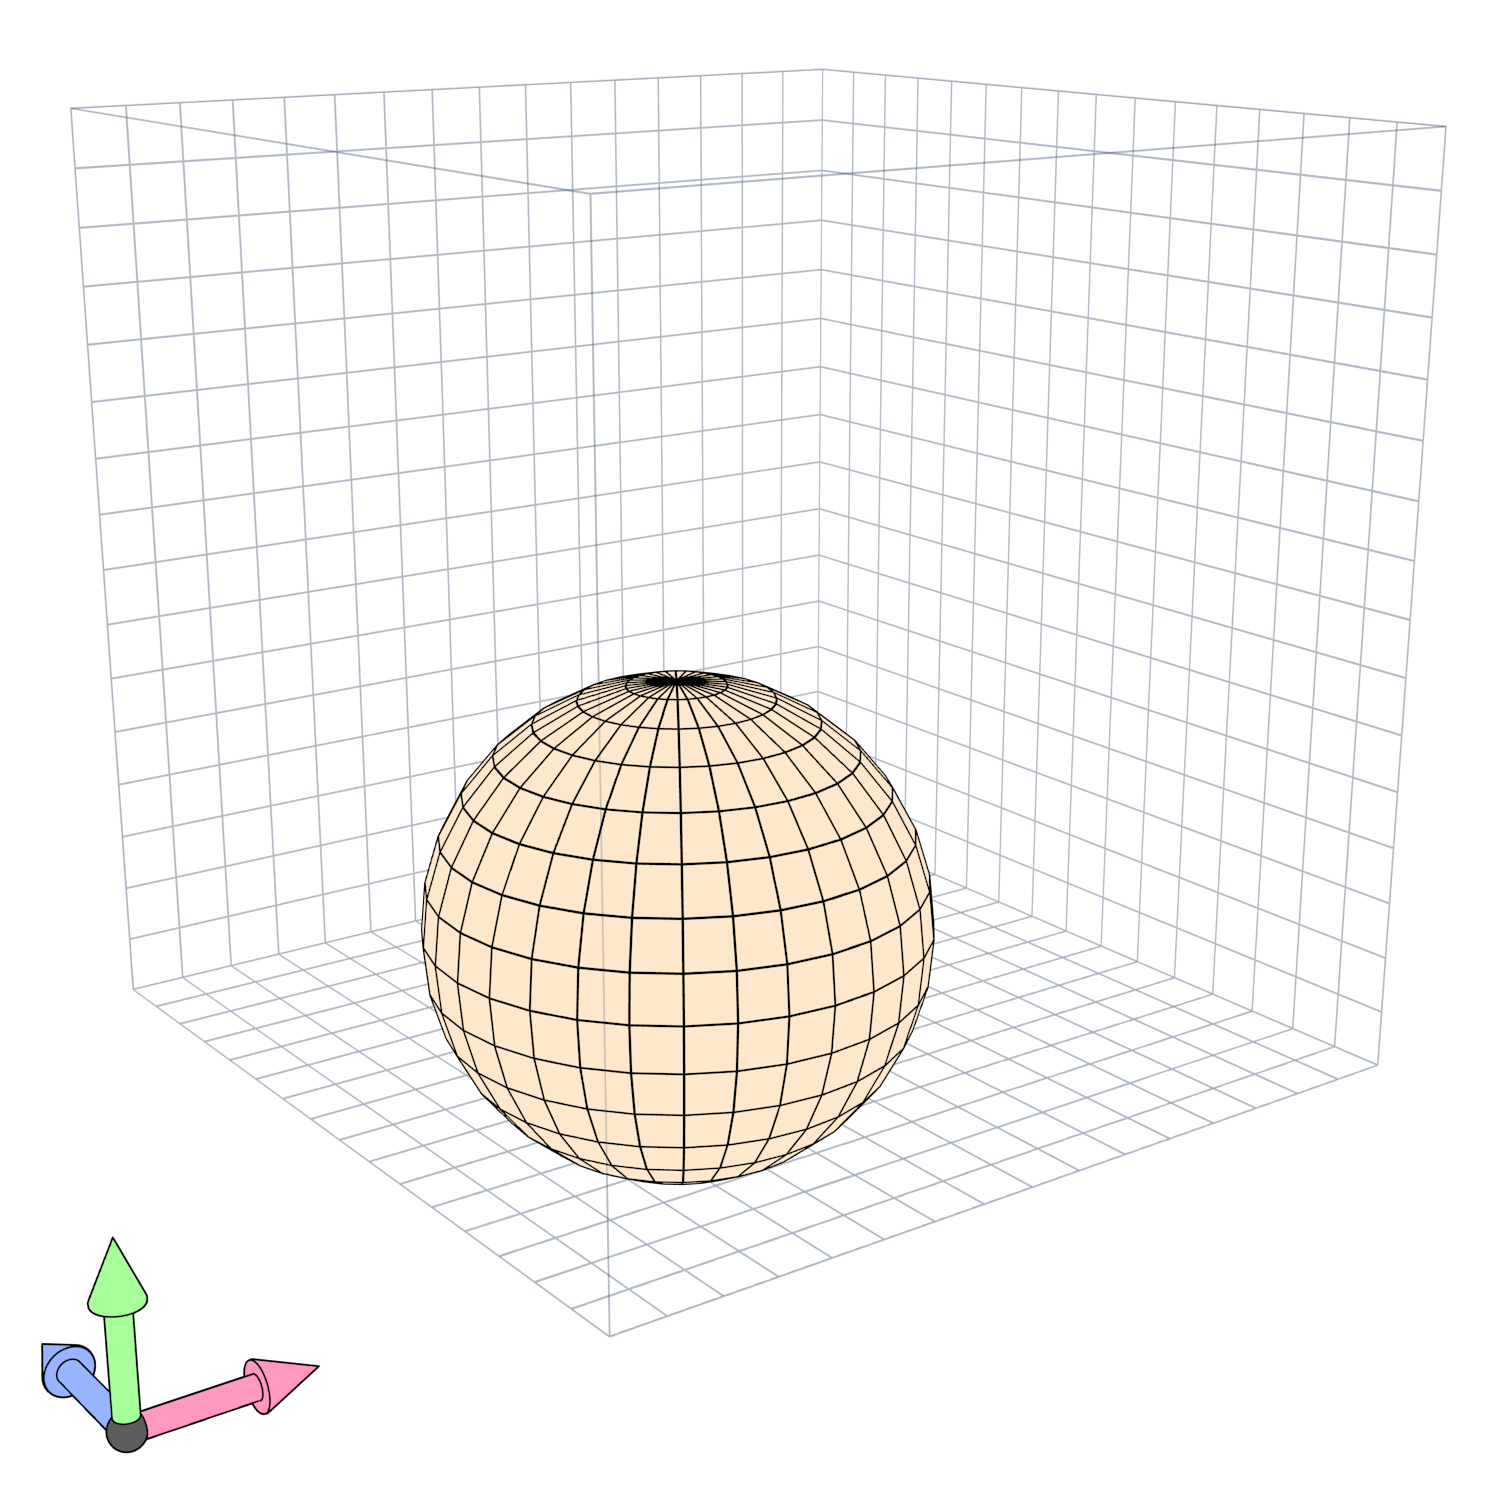
\includegraphics[width=\textwidth]{./img/raw/hs-slt/hs-slt_left.png}%
    \caption{Light volume}%
    \label{fig:hs-slt-left}%
  \end{subfigure} %
  \begin{subfigure}[b]{.45\linewidth}%
    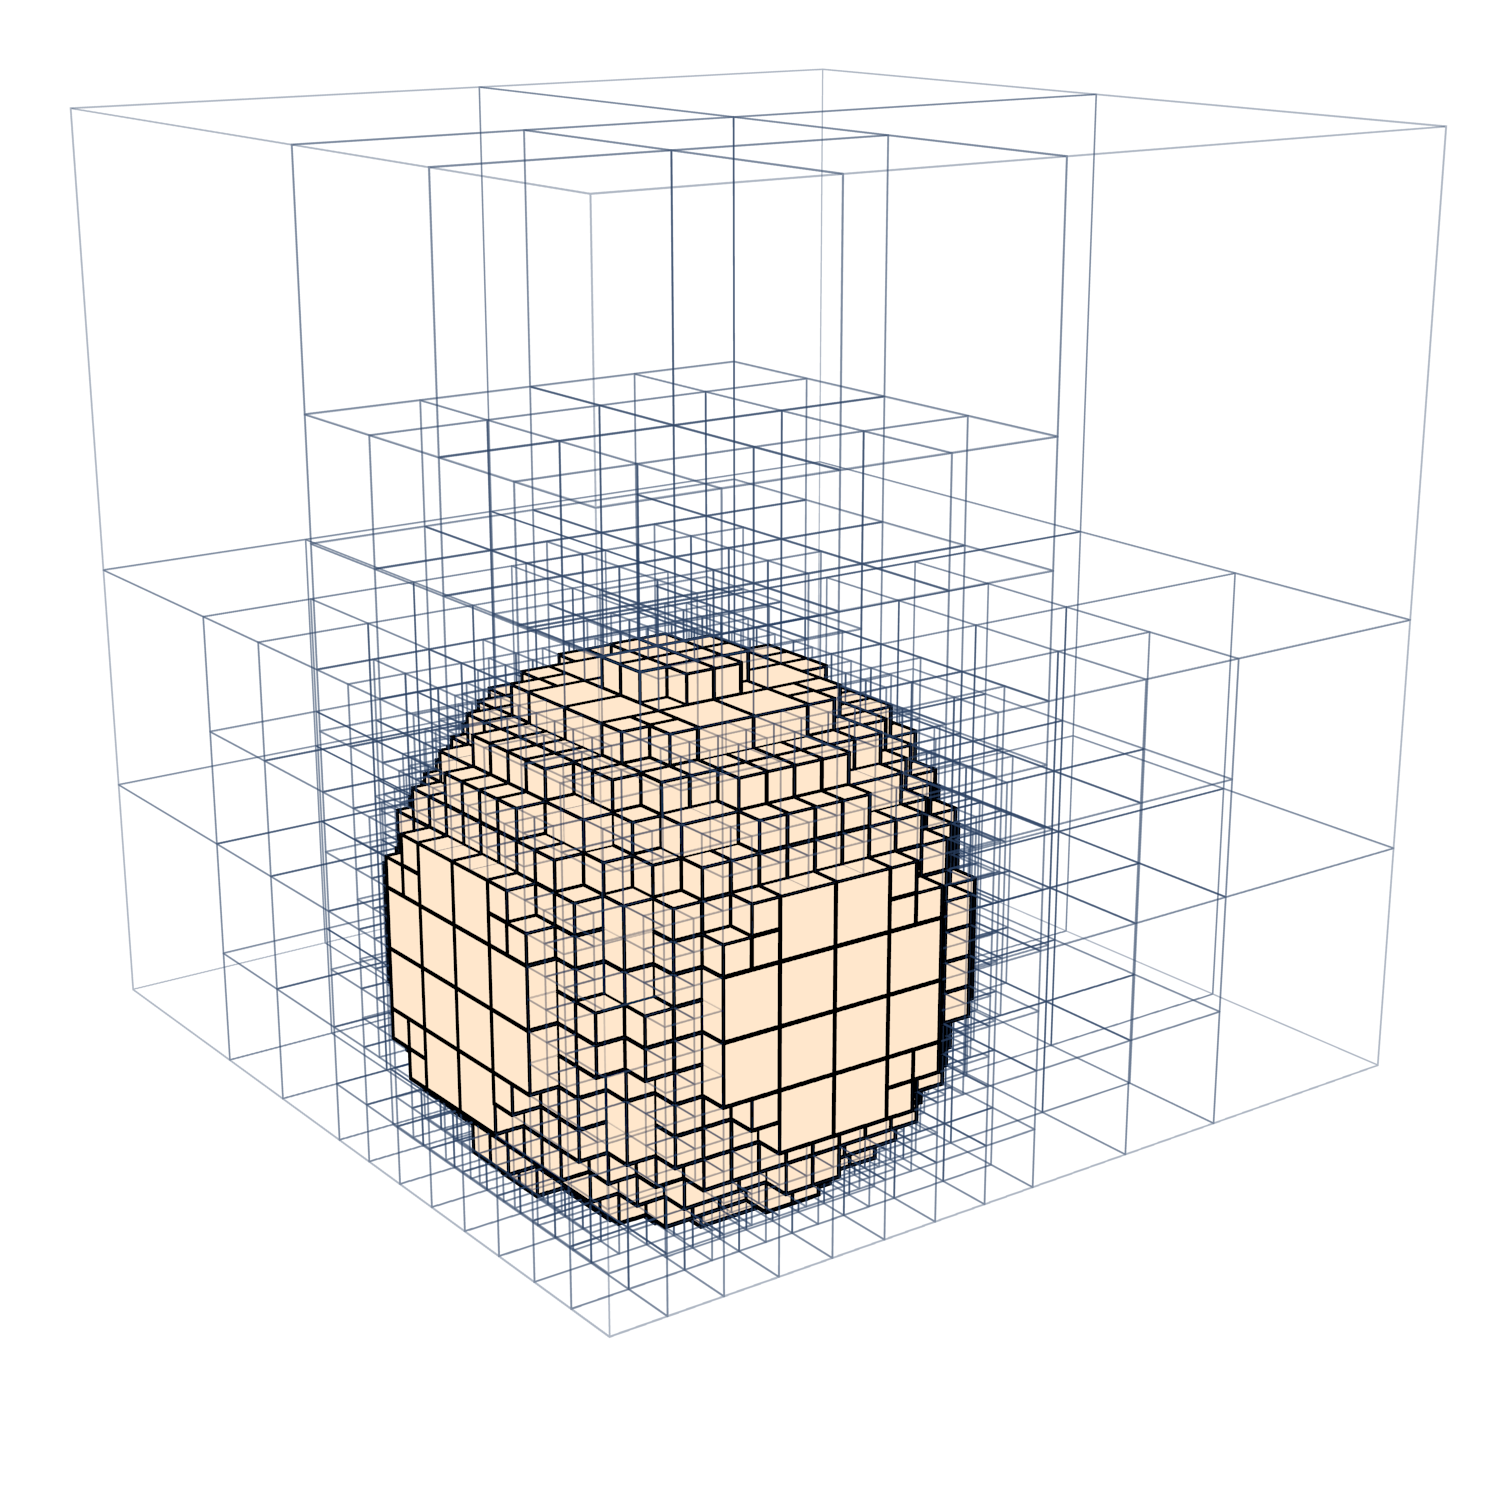
\includegraphics[width=\textwidth]{./img/raw/hs-slt/hs-slt_right.png}%
    \caption{Octree subdivision}%
    \label{fig:hs-slt-right}%
  \end{subfigure}
  \caption{Octree representation of a single light volume.}
  \label{fig:hs-slt}
\end{figure}


% Finally the way these lights are represented in memory needs to be considered. If a light is
% static during a whole simulation, there is no need to save the explicit influence of the
% light separately and the overlapping nodes can all be combined in the scene octree.
% However when a light is dynamic, the changing influence of the light on the subdivision of
% the scene space needs to be calculated. This can be done efficiently by comparing the nodes
% a light influences in the previous and current frame. Thus it is necessary to efficiently
% represent each dynamic light in memory, in order to save computation time.
% When the lights are small, or the node size is large, the grid could be saved directly in
% memory. However when the node size is small compared to the point light radius, this leads
% to unnecessary memory usage. The grid can be represented more compact by converting it into
% an octree as well. This can be done in a top-down fashion by making use of the grid.
% First the octree node which fully contains the grid is calculated. This node will serve
% as a root node. For each node there are initially three possible options. The grid
% does not overlap with the node, in which case the node is empty, as no overlapping nodes
% lay outside of the grid. The grid partially overlaps with the node and the node falls
% within the grid.

% When the node overlaps partially there are two possibilities. Either the grid node
% in the octree node closest to the light origin is overlapping, or it is not.
% If it is, then the octree node is a branch node, and the eight children are evaluated.
% If the grid node does not overlap with the light volume, the octree node is empty
% as well.

% In the last case there are three possibilities. If the grid node within the octree
% node volume closest to the light origin is empty, the octree node will be empty
% as well. If the closest grid node overlaps with the light volume, then either
% the grid node within the octree node volume furthest from the light origin overlaps
% with the light volume or it does not. In case it overlaps as well, then the whole
% octree node volume overlaps, and thus the octree node is an overlapping leaf node.
% If the furthest grid node does not overlap, the octree node contains both overlapping
% and non-overlapping nodes, and the octree node is a branch node. The children of
% this octree node are subsequently evaluated.

\subsection{Construction of the Scene Octree}

The scene octree combines the influences of the individual lights. Each leaf node
contains a set of references to the lights which overlap with the leaf node's volume.
This octree can be constructed either top-down or bottom-up, depending on the chosen
representation of the single lights.

In case the lights are represented by grid nodes, these nodes need to be combined such
that a set of nodes is obtained where each node contains the references to its overlapping
lights. Subsequently the shallower layers can be constructed. If eight sibling nodes share
the same set of indices they can be combined into a single leaf node in the proceeding
layer. If they are dissimilar a branch node is added to the proceding layer.

When the lights are represented by octrees, they can be added top-down to a scene
octree initialised with an empty leaf node. First the octree node corresponding with the
root node of the light is retrieved, constructing additional nodes where necessary.
Then each of the nodes of the light octree is added to the scene octree.

% The scene octree is an octree structure of which the leaf nodes contain references
% to the lights which overlap with the leaf node volumes. Depending on the representation
% of the single lights, the scene octree can be constructed either top-down or bottom-up.

% In case the lights are represented by the grid nodes which overlap with the light volume,
% the nodes need to be combined first. This creates a set of nodes of minimum size that contain a set of
% references to lights that overlap with these nodes. These can then be used to construct
% the octree bottom-up. If the eight sibling nodes are leaf nodes and contain the same set of indices, it can
% be replaced by a single leaf node in a higher layer, else a branch node in the layer above can be
% added.

% In case an octree representation is used, the scene octree can be build top-down by
% recursively adding the light octrees to the scene octree. For each light octree the
% scene octree node corresponding with the root of the light octree is found. Then the nodes
% of the light octree are recursively added, where the filled light octree nodes are added
% by adding the corresponding light index to the scene octree leaf node.

\subsection{Construction of the Linkless Octree and Light Index List}

The construction of the linkless octree follows the original algorithm. The
scene octree is represented by two spatial hash functions per layer, as only
nonempty leaf nodes have data associated with them. The first spatial hash function
describes the octree structure as described in the original algorithm. The second spatial
hash function contains a data element consisting of two integers per nonempty leaf node.
These integers specify the subset of light indices within the Light Index List that
describe the lights which overlap with the leaf node.

In order to construct this linkless octree, the nodes of the specified starting depth
are gathered. For each of these nodes the octree node encoding is calculated. If a
node is a nonempty leaf node, the current length of the Light Index List and the size of
the set of lights associated with the leaf node are added to the second spatial hash function,
as the offset and the length values respectively. The light indices of the set of lights
are then added to the Light Index list.

Once all layers have been constructed, the linkless octree and the Light Index List can
be loaded into GPU memory.

% As described in the overview, the octree nodes will specify a subset of the light index list.
% Because this data is only saved in the leaf nodes of the scene octree. We opted for the
% linkless octree variant that saves the data of the octree nodes separately from the octree
% structure. Thus per layer a maximum of two spatial hash functions is constructed.

% In the first step of construction of the linkless octree and light index list, the scene
% octree nodes at the specified starting depth are gathered. For each of these nodes the
% octree structure value is calculated as is specified in the algorithm of the linkless octree.
% For each node we save whether the node is a leaf node, and whether the node contains any
% information. If a node contains information, this information is stored in the second
% spatial hash function. For each non-empty leaf node, the length of light index list
% is saved, then the indices associated with the leaf node are added to the light index list.
% The value saved in the second spatial hash function specifies the offset, equal to the length
% of the light index list before adding the indices, and the length of the set of light indices.

\subsection{Light Assignment during Shading}

The final step of the algorithm is to determine the set of relevant lights for the samples
generated during rendering. This step is similar to that of Tiled and Clustered Shading.
First the leaf node containing the sample has to be calculated by descending into
the octree until a leaf node is encountered. If this leaf node is nonempty then the
offset and length can be retrieved from the corresponding data hash table. Else a length of
zero is returned. Once the offset and length are retrieved the set of light indices
from the Light Index List can be obtained. The sample is then shaded by summing the
shading contributions of the corresponding lights. This step is equal to that of
Tiled and Clustered Shading.

% The final step of the algorithm is to use the constructed data structures to determine the set
% of relevant lights per sample during the shading step. This step is similar to the shading
% step of both Tiled and Clustered Shading. In order to find the subset of indices within the
% light index list for a sample, we need to descend into the octree. For each layer we
% calculate the octree structure of the node in which the sample falls. If this is a branch node,
% the next layer is calculated. If the scene octree node is an empty leaf node, a vector containing
% two zeroes is returned. If the the scene octree node is non-empty, the corresponding value is
% obtained from the second spatial hash function of the current layer. The found offset and length
% are returned.

% Once the offset and length are obtained, the algorithm loops over the light indices within
% the light index list, and for each light calculates the light contribution to the sample.
% These values are summed and saved for the particular sample.

